\begin{enumerate}
    \item \emph{addressing} -- Nodes are identified by their \gloss{underlay address}.
    \item \emph{dialling} -- Nodes can initiate a direct connection to a peer by dialing them on their underlay address.
    \item \emph{listening} -- Nodes can listen to other peers dialing them and can accept incoming connections. Nodes that do not accept incoming connections are called \glossplural{light node}.
    \item \emph{live connection} -- A node connection establishes a channel of communication which is kept alive until explicit disconnection, so that the existence of a connection means the remote peer is online and accepting messages.
    \item \emph{channel security} -- 
    The channel provides identity verification and implements encrypted and authenticated transport resisting man in the middle attacks.
    \item \emph{protocol multiplexing} -- 
    The underlay network service can accommodate several protocols running on the same connection. Peers communicate the protocols with the name and versions that they implement and the underlay service identifies compatible protocols and starts up peer connections on each matched protocol. 
    \item \emph{delivery guarantees} -- 
    Protocol messages have \gloss{guaranteed delivery}, i.e. delivery failures due to network problems result in direct error response. 
    Order of delivery of messages within each protocol is guaranteed. 
    Ideally the underlay protocol provides prioritisation. 
    If protocol multiplexing is over the same transport channel, this most likely implies framing, so that long messages do not block higher priority messages.
    \item \emph{serialisation} -- 
    The protocol message construction supports arbitrary data structure serialisation conventions.
    
\end{enumerate}

The \gloss{libp2p} library can provide all the needed functionality and is the one given in the specification as underlay connectivity driver, see \ref{spec:protocol:intro}.%
%
\footnote{Swarm's initial golang implementation uses Ethereum's \gloss{devp2p}/rlpx which satisfies the above criteria and uses TCP/IP with custom cryptography added for security. The underlay network address that devp2p uses is represented using the \gloss{enode URL scheme}. Devp2p dispatches protocol messages based on their message ID. It uses RLP serialisation which is extended with higher level data type representation conventions. In order to provide support for the Ethereum 1.x blockchain and for storing its state on Swarm, we may provide a thin devp2p node that proxies queries to the new libp2p-based Swarm client, or just uses its API. Otherwise we expect the devp2p networking support to be discontinued.}

\subsection{Overlay addressing\statusgreen}\label{sec:overlay-addressing} 
\green{}

While clients use the \gloss{underlay address} to establish connections to peers, each node running Swarm is additionally identified with an \gloss{overlay address}. It is this address that determines which peers a node will connect to and directs the way that messages are forwarded. The overlay address is assumed to be stable as it defines a nodes' identity across sessions and ultimately affects which content is most worth storing in the nodes' local storage.

The node's \gloss{overlay address} is derived from an Ethereum account by hashing the corresponding elliptic curve public key with the \gloss{BZZ network ID}, using the 256-bit Keccak algorithm (see \ref{spec:format:bzzaddress}). The inclusion of the BZZ network ID stems from the fact that there can be many Swarm networks (e.g.\ test net, main net, or private Swarms). Including the BZZ network ID makes it impossible to use the same address across networks. Assuming any sample of base accounts independently selected, the resulting overlay addresses are expected to have a uniform distribution in the address space of 256-bit integers. It is important to derive the address from a public key as it allows the nodes to issue commitments associated with an overlay location using cryptographic signatures that are verifiable by 3rd parties. 

Using the long-lived communication channels of the \gloss{underlay network}, Swarm nodes form a network with \emph{quasi-permanent} peer connections. The resulting connectivity graph can then realise a particular topology defined over the address space. The \gloss{overlay topology} chosen is called \gloss{Kademlia}: It enables communication between any two arbitrary nodes in the Swarm network by providing a strategy to relay messages using only underlay peer connections. The protocol that describes how nodes share information with each other about themselves and other peers, called 'Hive' is described in \ref{spec:protocol:hive}. How nodes use this protocol to bootstrap the \gloss{overlay topology} is discussed in \ref{sec:bootstrapping}. The  theoretical basis for \gloss{Kademlia topology} is formalised rigorously in \ref{sec:kademlia-connectivity}. 

Crucially, the overlay address space is all 256-bit integers. Central to Swarm is the concept of \gloss{proximity order} (\gloss{PO}), which quantifies the relatedness of two addresses on a discrete scale.%
%
\footnote{Proximity order is the discrete logarithmic scale of proximity, which, in turn is the inverse of normalised XOR distance. See \ref{sec:proximity} for a formal definition.}
%
Given two addresses, $x$ and $y$, $\mathit{PO}(x,y)$ counts the matching bits of their binary representation starting from the most significant bit up to the first one that differs. The highest proximity order is therefore 256, designating the maximum relatedness, i.e. where $x=y$.

\subsection{Kademlia routing \statusgreen}\label{sec:kademlia-routing}
\yellow{rework together with appendix}

\glossupper{Kademlia topology} can be used to route messages between nodes in a network using overlay addressing. It has excellent scalability as it allows for a universal routing such that both (1) the number of hops and (2) the number of peer connections are always logarithmic to the size of the network. 

In what follows, we show the two common flavours of routing: \emph{iterative/zooming} and \emph{recursive/forwarding}. Swarm's design crucially relies on choosing the latter, the forwarding flavour. However, this is unusual, and, as the iterative flavour predominates within much of the peer-to-peer literature and most other implementations are using iterative routing  (see \cite{maymounkov2002kademlia,baumgart2007s,lua2005survey}), we consider it useful to walk the reader through both approaches so their idiosyncrasies may be revealed.

\subsubsection{Iterative and forwarding Kademlia}

Let $R$ be an arbitrary binary relation over nodes in a network. Nodes that are in relation $R$ with a particular node $x$ are called \glossplural{peer} of $x$. Peers of $x$ can be indexed by their \gloss{proximity order} (\gloss{PO}) relative to $x$ (see \ref{sec:proximity}).
The equivalence classes of peers are called \glossplural{proximity order bin}, or just bins for short. Once arranged in bins, these groups of peers form the \gloss{Kademlia table} of the node $x$ (see figure \ref{fig:kademlia-table}). 



\begin{figure}[htbp]
   \centering
    % \includegraphics[width=0.7\textwidth]{fig/kademlia.pdf}
    % \includegraphics[width=0.7\textwidth]{fig/kademlia-2.pdf}
    % 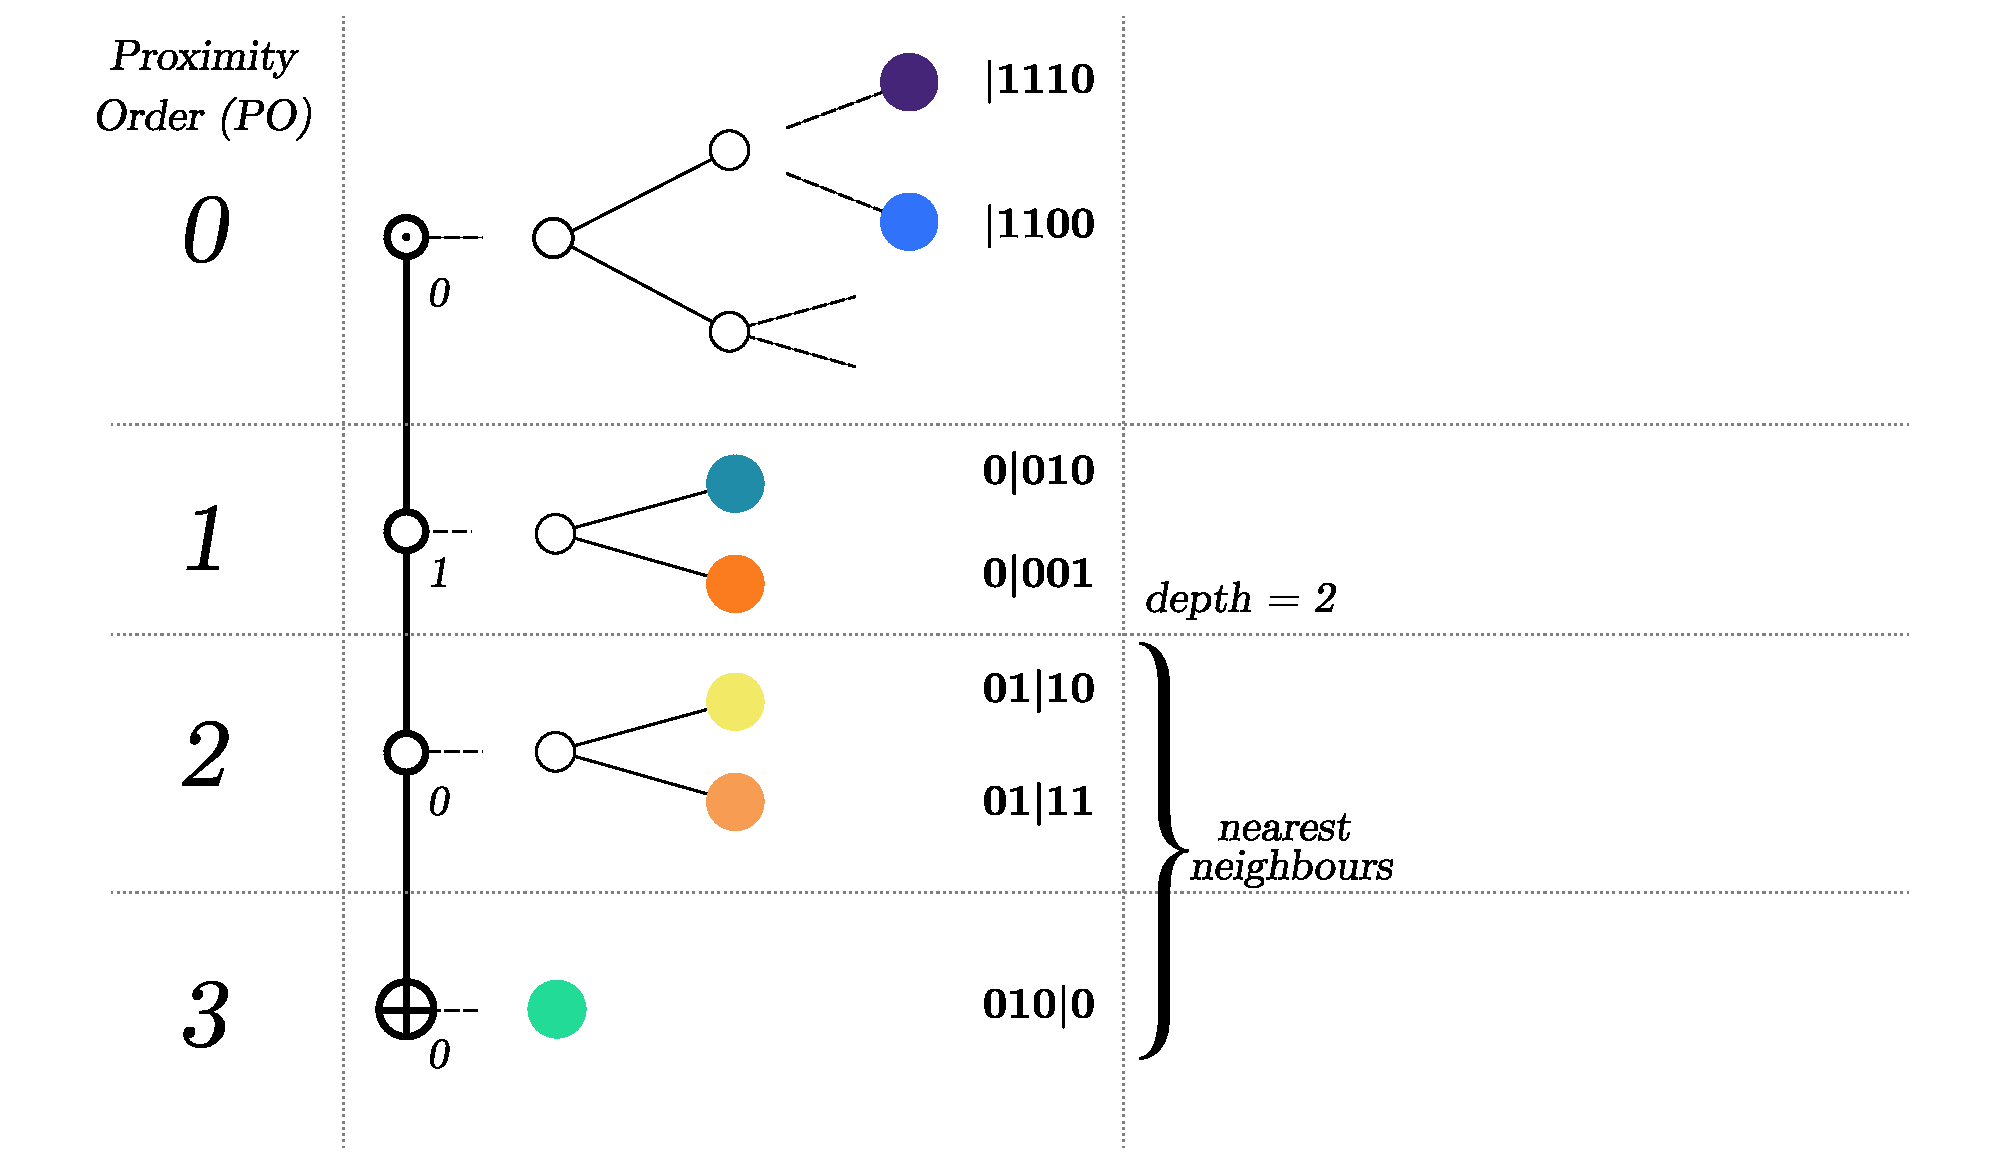
\includegraphics[width=0.8\textwidth]{fig/kademlia-3.pdf}
    \includegraphics[width=.88\textwidth]{fig/kademlia-35.pdf}
   \caption[From overlay address space to Kademlia table \statusgreen]{From overlay address space to Kademlia table. \textbf{Top}: the overlay address space is represented with a binary tree, colored leaves are actual nodes. The path of the pivot node (+) is shown with thicker lines. \textbf{Centre}: peers of the pivot nodes are shown keyed by the bits of their xor distance measured from the pivot. Here zeros represent a matching bit with the pivot, ones show a differing bit. The leaf nodes are ordered by their xor distance from the pivot (leftmost node). \textbf{Bottom}: the Kademlia table of the pivot: the subtrees branching off from the pivot path on the left are displayed as the rows of the table representing proximity order bins in increasing order.}
   \label{fig:kademlia-table}
\end{figure}

Node $x$ has a \gloss{saturated Kademlia table} if there is a $0\leq d_x\leq \mathit{maxPO}$ called the  \gloss{neighbourhood depth} such that (1) the node has at least one peer in each bin up to and excluding \gloss{proximity order} bin $d_x$ and (2) all nodes at least as near as $d_x$ (called the \gloss{nearest neighbours}) are peers of $x$. If each node in a network has a saturated Kademlia table, then we say that the network has \gloss{Kademlia topology}.

\begin{figure}[htbp]
   \centering
    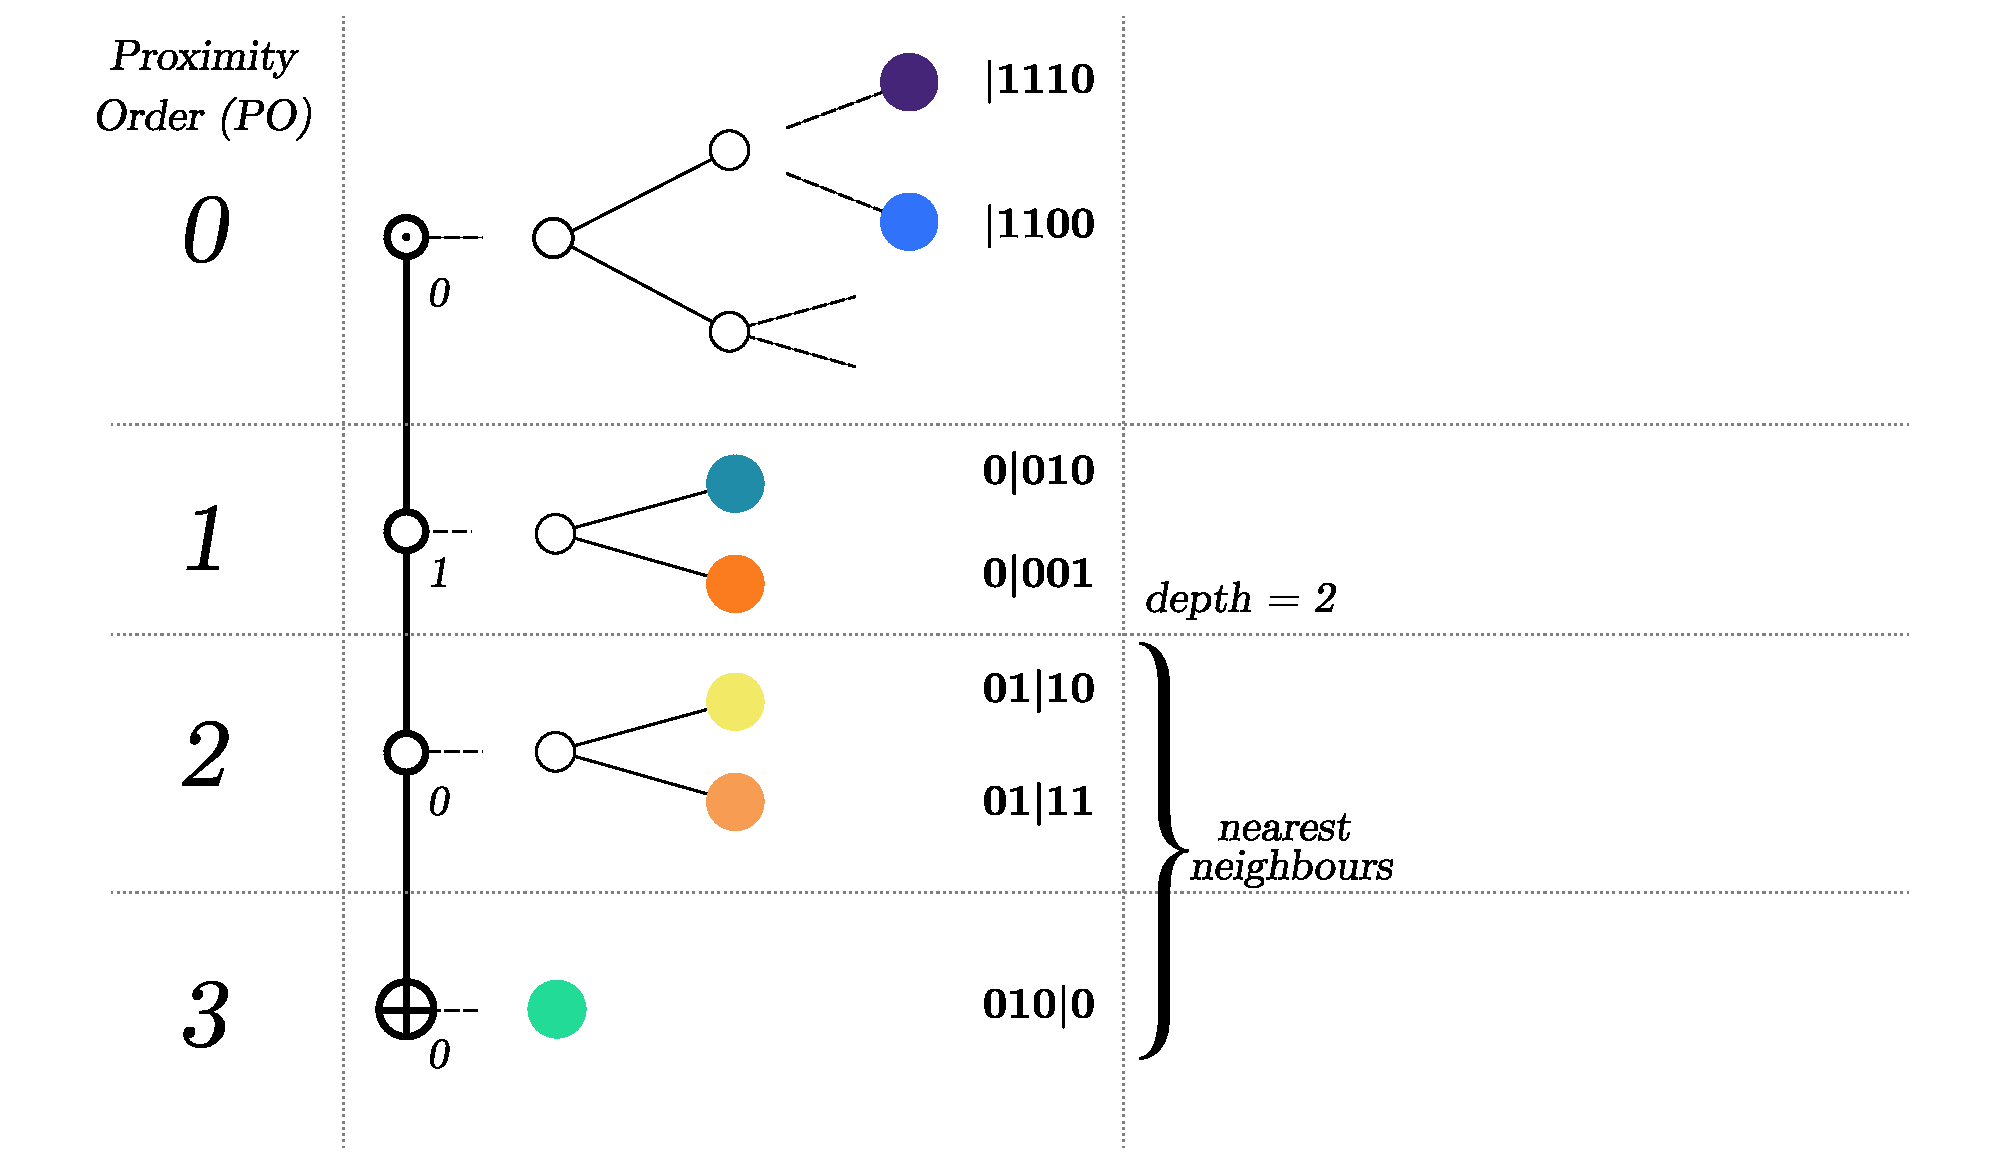
\includegraphics[width=\textwidth]{fig/kademlia-3.pdf}
   \caption[Nearest neighbours \statusgreen]{Nearest neighbours in a 4 bit network with $d = 2$ }
   \label{fig:bin-density}
\end{figure}

Let $R$ be the "is known to" relation:  $y$ "is known to" $x$ if $x$ has both overlay and underlay addressing information for $y$. 
In the iterative Kademlia routing the \gloss{requestor node} iteratively extends the graph of peers that are known to it. Using their \gloss{underlay address}, the requestor node will contact the peers that they know are nearest the destination address for peers that are further away (commonly using UDP), on each successive iteration the peers become at least one order closer to the destination (see figure \ref{fig:iterative-forwarding-kademlia}). Because of the Kademlia criteria, the requestor will end up eventually discovering the destination node's underlay address and can then establish direct communication with it. This iterative strategy%
%
\footnote{The iterative protocol is equivalent to the original Kademlia routing that is described in \cite{maymounkov2002kademlia}.
}
%
critically depends on the nodes' ability to find peers that are currently online. In order to find such a peer, a node needs to collect several candidates for each bin. The best predictor of availability is the recency of the peer's last response, so peers in a bin should be prioritised according to this ordering.

\begin{figure}[htbp]
   \centering
   \vspace{-2cm} 
   \includegraphics[width=.8\textwidth]{fig/iterative-kademlia.pdf}\\\vspace{-1.3cm}
   \includegraphics[width=.8\textwidth]{fig/forwarding-kademlia-3.pdf}
   \caption[Iterative and Forwarding Kademlia routing \statusgreen]{Iterative and Forwarding Kademlia routing: A requestor node shown with a cross in the circle at address $...0000...$ wants to route to a destination address $...1111...$ to which the closest peer online is the blue circle at $...1110...$ These initial ellipses represent the prefix shared by requestor and destination addresses which is $n$ bits long. \textbf{Top:} In the iterative flavour, the requestor contacts the peers (step 1, dotted black arrows) that they know are nearest the destination address. Peers that are online (yellow) respond with information about nodes that are even closer (green arrow, step 2) so the requestor can now repeat the query using these closer peers (green, step 3). On each successive iteration the peers (yellow, green and blue) are at least one PO closer to the destination until eventually the requestor is in direct contact with the node that is nearest to the destination address. \textbf{Bottom:} In the forwarding flavour, the requestor forwards a message to the connected peer they know that is nearest to the destination (yellow). The recipient peer does the same. Applying this strategy recursively relays the message via a chain of peers (yellow, green, blue) each at least one PO closer to the destination.}
   \label{fig:iterative-forwarding-kademlia}
\end{figure}


Swarm uses an alternative flavour of Kademlia routing which is first described in \cite{heep2010r} and then expanded on and worked out in \cite{tronetal2019-network}. Here, a recursive method is employed, whereby the successive steps of the iteration are "outsourced" to a \gloss{downstream peer}.
Each node recursively passes a message to a direct peer at least one \gloss{proximity order} closer to the destination. Thus, \gloss{routing} using this approach, simply means relaying messages via a chain of peers which are ever closer to the destination, as shown in figure \ref{fig:iterative-forwarding-kademlia}.


In this way, Swarm's underlay transport offers quasi-stable peer connections over TCP with communication channels that are kept alive. These open connections can then be used as $R$ to define another notion of a \gloss{peer}. The two criteria of healthy \gloss{Kademlia connectivity} in Swarm translate as: For each node $x$, there exists a \gloss{neighbourhood depth} $d_x$ such that (1) node $x$ has an open connection with at least one node for each \gloss{proximity order bin} up to but excluding $d_x$ and (2) is connected to all the online nodes that are at least as near as $d_x$. If each node in the network has a saturated Kademlia table of peers, then the network is said to have \gloss{Kademlia topology}. Since connected peers are guaranteed to be online, the recursive step consists solely of forwarding the message to a connected peer strictly closer to the destination. We can call this alternative a \gloss{forwarding Kademlia}.


In a \gloss{forwarding Kademlia} network, a message is said to be \emph{routable} if there exists a path from sender to destination through which the message can be relayed. In a mature subnetwork with \gloss{Kademlia topology} every message is routable. 

If all peer connections are stably online, a \gloss{thin Kademlia table}, i.e.\ a single \gloss{peer} for each bin up to $d$, is sufficient to guarantee routing between nodes. In reality, however, networks are subject to \gloss{churn}, i.e.\ nodes are expected to go offline regularly. In order to ensure \gloss{routability} in the face of churn, the network needs to maintain \gloss{Kademlia topology}. This means that each individual node needs to have a \gloss{saturated Kademlia table} at all times. By keeping several connected peers in each \gloss{proximity order bin}, a node can ensure that node dropouts do not damage the saturation of their Kademlia table. Given a model of node dropouts, we can calculate the minimum number of peers needed per bin to guarantee that nodes are saturated with a probability that is arbitrarily close to 1. The more peers a node keeps in a particular proximity order bin, the more likely that the message destination address and the peer will have a longer matching prefix. As a consequence of forwarding the message to that peer, the \gloss{proximity order} increases more quickly, and the message ends up closer to the destination than it would with less peers in each bin (see also figure \ref{fig:bindensity}).



With \gloss{Kademlia} saturation guaranteed, a node will always be able to forward a message and ensure \gloss{routability}. If nodes comply with the forwarding principles (and that is ensured by \gloss{aligned incentives}, see \ref{spec:strategy:forwarding}) the only case when relaying could possibly break down is when a node drops out of the network after having received a message but before it managed to forward it.%
%
\footnote{Healthy nodes could commit to being able to forward within a (very short) constant time; let's call this the \gloss{forwarding lag}. In the case that a \gloss{downstream peer} disconnects before this forwarding lag passes, then the \gloss{upstream peer} can re-forward the message to an alternative peer, thereby keeping the message passing unbroken. See \ref{sec:retrieval} for more detail.
} 

An important advantage of forwarding Kademlia is that this method of routing requires a lot less bandwidth than the iterative algorithm. In the iterative version, known peers are not guaranteed to be online, so finding one that is adds an additional level of unpredictability.

\subsubsection{Sender anonymity}
\glossupper{sender anonymity} is a crucial feature of Swarm. It is important that peers further down in the request cascade can never know who the originator of the request was, because requests are relayed from peer-to-peer. 

The above rigid formulation of Kademlia routing would suggest that if a node receives a message from a peer and that message and peer have a proximity order of $0$, then the recipient would be able to conclude that the peer it received the message from must be the sender. If we allow \gloss{light node} Swarm clients, i.e. clients that due to resource constraints do not keep a full Kademlia saturation but instead have just a local neighbourhood, then even a message from a peer in bin $0$ remains of ambiguous origin. 

\subsubsection{Bin density and multi-order hops} \label{sec:bindensity}

As a consequence of logarithmic distance and uniform node distribution, farther peers of a particular node are exponentially more numerous. 
This means that unless the number of required connections in a bin doubles as bins go farther from the node, shallower bins will always allow more choice of nodes for potential connection. In particular, nodes have a chance to increase the number of connections per bin in such a way that peer addresses maximise density (i.e., in proximity order bin $b$, the subsequent bits of peer addresses form a \gloss{balanced binary tree}). Such an arrangement is optimal in the sense that for a bin depth of $d$, nodes are able to relay all messages so that in one hop the proximity order of the destination address will increase by $d$ (see figure \ref{fig:bindensity}). 


\begin{figure}[htbp]
   \centering
   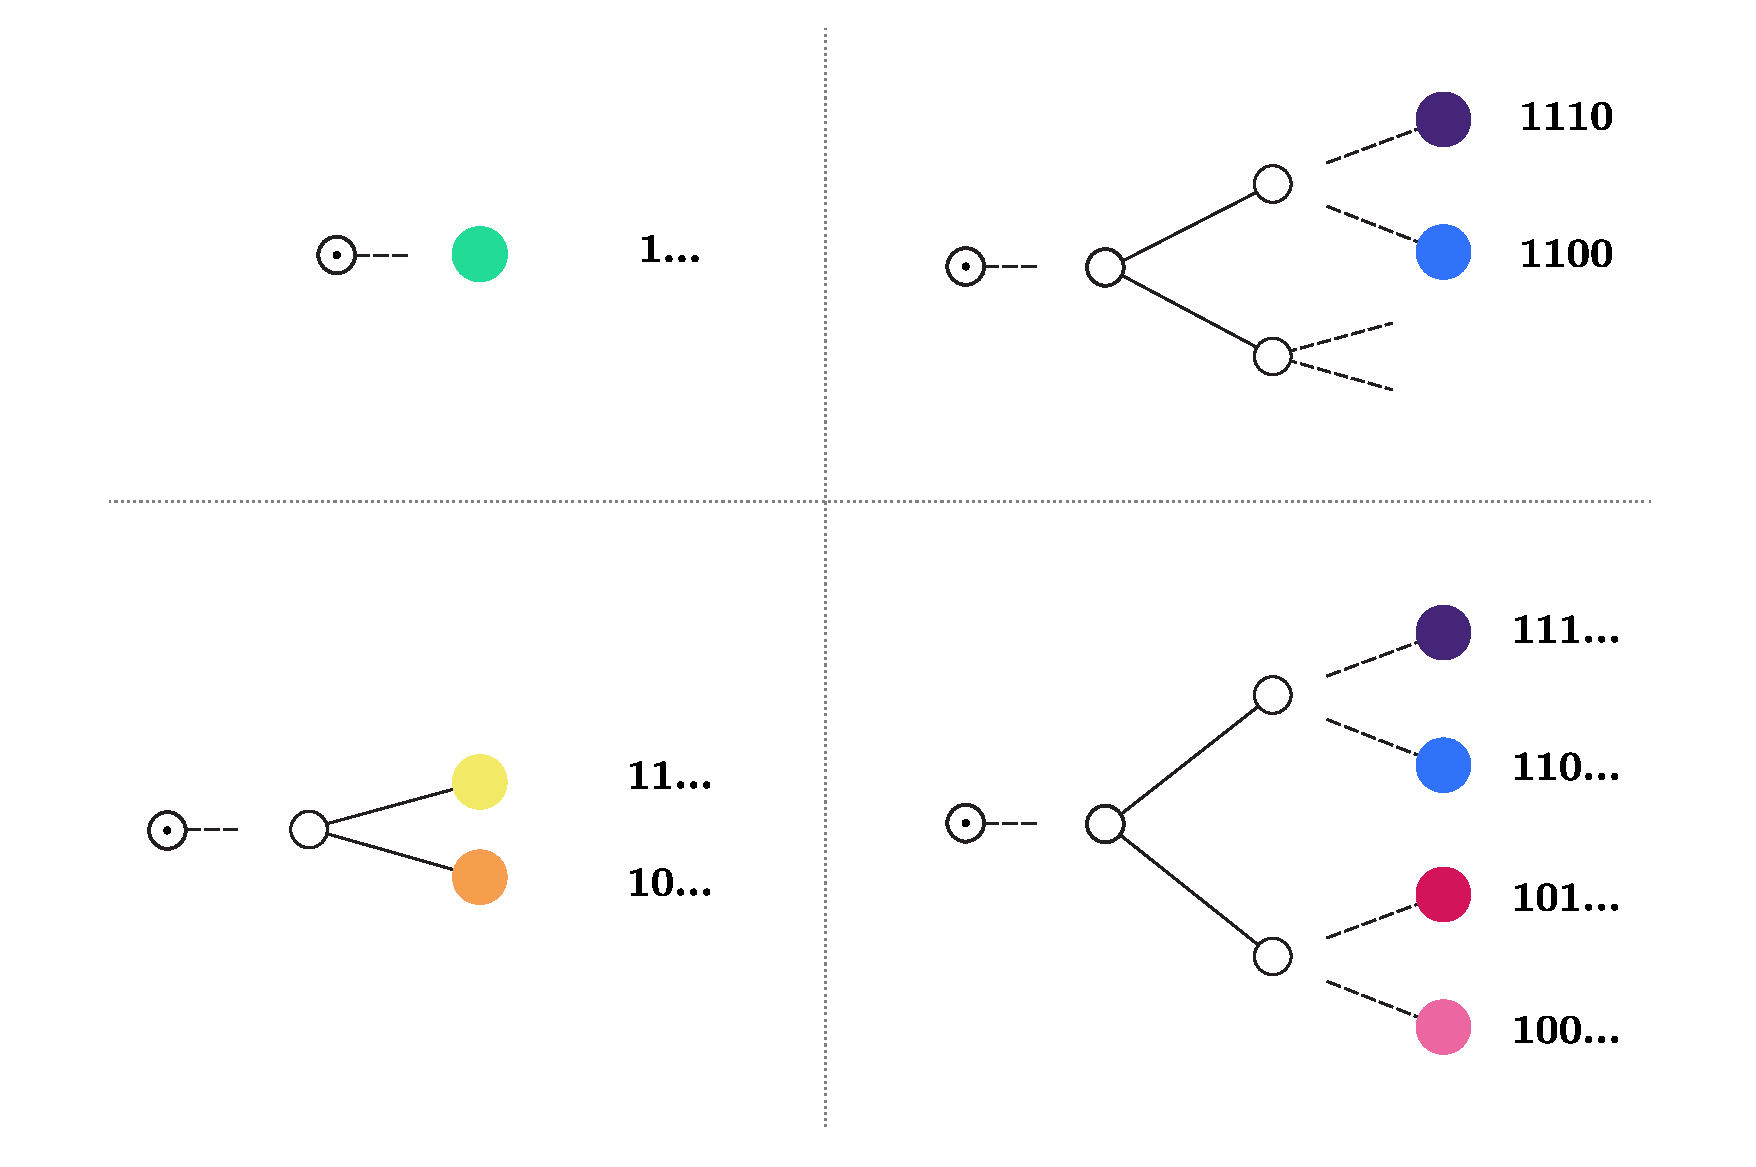
\includegraphics[width=\textwidth]{fig/bindensity.pdf}
   \caption[Bin density \statusgreen]{Bin density:  types of saturation for PO bin $0$ for a node with overlay address starting with bit $0$. \textbf{Top left}: A "thin" bin with a single peer is not resilient to churn and only increases PO by $1$ in one hop. \textbf{Top right:} At least two peers are needed to maintain Kademlia topology in case of churn; two peers when not balanced cannot guarantee multi-order hops. \textbf{Bottom left:} Two peers balanced guarantees an increase of 2 PO-s in one hop. \textbf{Bottom right:} Four peers when balanced can guarantee an increase of $3$ PO-s in one hop.}
   \label{fig:bindensity}
\end{figure}

\subsubsection{Factoring in underlay proximity}
It is expected that as Swarm clients continue to evolve and develop, nodes may factor in throughput when they select peers for connection. All things being equal, nodes physically closer to each other tend to have higher throughput, and therefore will be preferred in the long run. This is how forwarding Kademlia is implicitly aware of underlay topology \cite{heep2010r}. See \ref{spec:strategy:connection} for a more detailed discussion of connectivity strategy.


\subsection{Bootstrapping and maintaining Kademlia topology \statusgreen}\label{sec:bootstrapping}
 
\orange{rework based on new hive protocol}
 
This section discusses how a stable Kademlia topology can emerge. In particular, the exact bootstrapping protocol that each node must follow to reach and maintain a saturated Kademlia connectivity. Nodes joining a \gloss{decentralised network} are supposed to be initially naive, potentially initiating connection via only a single known peer with no prior knowledge. For this reason, the bootstrapping process needs to include an initial step that helps naive nodes to begin exchanging information about each other. This discovery process is called the \gloss{hive protocol} and is formally specified in \ref{spec:protocol:hive}.

\subsubsection{Bootnodes}

Swarm has no distinct node type or operation mode for bootnodes. This means that naive nodes should be able to connect to any node on the  network and bootstrap their desired connectivity. In order not to overburden any single node, electing one particular node as an initial connection should be avoided, and the role of being a bootnode for the newly connecting naive nodes should ideally be distributed among participant nodes. This is achieved either with an invite system, or a centralised bootnode service running a public gateway that responds to an API call with the bzz address of a randomly chosen node among online peers. 

Once connected to a node in the network, the hive protocol kicks in and the naive node begins to learn about the bzz addresses of other nodes, and thus it can start bootstrapping its connectivity.

\subsubsection{Building up connections}

Initially, each node begins with zero as their \gloss{saturation depth}. Nodes keep advertising their saturation depth to their connected peers as it changes. When a node $A$ receives an attempt to establish a new connection from a node $B$, she notifies each of her other peers about $B$ connecting to her only in the case that each peer's proximity order relative to the connecting node $A$ is not lower than that peer's advertised saturation depth. The notification is always sent to a peer that shares a proximity order bin with the new connection. Formally, when $y$ connects to $x$, $x$ notifies a subset of its connected peers. A peer $p$ belongs to this subset if $\mathit{PO}(x, p) = \mathit{PO}(x, y)$ or $d_p\leq \mathit{PO}(y, p)$. The notification takes the form of a protocol message and includes the full \gloss{overlay address} and \gloss{underlay address} information (see \ref{spec:format:bzzaddress}).%
%
\footnote{Light nodes that do not wish to relay messages and do not aspire to build up a healthy Kademlia, are not included, see section \ref{sec:light}. }

    

% \begin{figure}[htbp]
%   \centering
%   \caption[Hive protocol: bootstrapping and maintaining Kademlia topology \statusred]{Hive protocol: bootstrapping and maintaining Kademlia topology}
%   \label{fig:bootstrapping-kademlia}
% \end{figure}

\subsubsection{Mature connectivity}

After a sufficient number of nodes are connected, a bin becomes saturated, and the node's neighbourhood depth can begin to increase. Nodes keep their peers up to date by advertising their current depth if it changes. As their depth increases, nodes will get notified of fewer and fewer peers. Once the node finds all their nearest neighbours and has saturated all the bins, no new peers are to be expected. For this reason, a node can conclude a saturated Kademlia state if it receives no new peers for some time.%
%
\footnote{Note that the node does not need to know the total number of nodes in the network. In fact, some time after the node stops receiving new peer addresses, the node can effectively estimate the size of the network: the depth of network is $\log_2(n+1)+ d$ where $n$ is the number of remote peers in the nearest neighbourhood and $d$ is the depth of that neighbourhood. It then follows that the total number of nodes in the network can be estimated simply by taking this to the power of 2.}
%
Instead of having a hard deadline and a binary state of saturation, we can quantify the certainty of saturation by the age of the last new peer received. Assuming stable connections, eventually each node online will get to know its nearest neighbours and connect to them while keeping each bin up to $d$ non-empty. Therefore each node will converge on the saturated state. If no new nodes join, health (Kademlia topology) is maintained even if peer connections change. A node is not supposed to go back to a lower saturation state for instance. This is achieved by requiring several peers in each proximity order bin. 

\section{Swarm storage\statusgreen}\label{sec:kademlia-storage}

In this section, in \ref{sec:disc}, we first show how a network with quasi-permanent connections in a Kademlia topology can support a \gloss{load balancing}, \gloss{distributed storage} of fixed-sized datablobs. In \ref{sec:chunks}, we detail the generic requirements on chunks and introduce actual chunk types. Finally, in \ref{sec:redundancy-by-local-replication}, we turn to \gloss{redundancy} by neighbourhood replication as a first line of defense against node churn.

\subsection{Distributed immutable store for chunks\statusgreen}\label{sec:disc}
 
In this section we discuss how networks using Kademlia overlay routing are a suitable basis on which to implement a serverless storage solution using \glossplural{distributed hash table} (\glossplural{DHT}). Then we introduce the \gloss{DISC}%
%
\footnote{DISC is \gloss{distributed immutable store for chunks}. In earlier work, we have referred to this component as the 'distributed preimage archive' (DPA), however, this phrase became misleading since we now also allow chunks that are not the preimage of their address.}
% 
model, Swarm's narrower interpretation of a DHT for storage. This model 
imposes some requirements on chunks and necessitates 'upload' protocols. 

As is customary in Swarm, we provide a few resolutions of this acronym, which summarise the most important features:


\begin{itemize}
\item \emph{decentralised infrastructure for storage and communication}, 
\item \emph{distributed immutable store for chunks}, 
\item \emph{data integrity by signature or content address},
% \item \emph{downloadable incentivised secure communications}
\item \emph{driven by incentives with smart contracts}. 

\end{itemize}
 
\subsubsection{From DHT to DISC}
Swarm's \gloss{DISC} shares many similarities with the wider known \glossplural{distributed hash table}. The most important difference is that Swarm does not keep track of \emph{where} files are to be found, instead it actually \emph{stores pieces of the file itself} directly with the closest node(s). 
In what follows, we review DHTs, as well as dive into the similarities and differences with DISC in more detail. 
 
\glossupperplural{distributed hash table} use an overlay network to implement a key--value container distributed over the nodes (see figure \ref{fig:DHT}). The basic idea is that the keyspace is mapped onto the overlay address space, and the value for a key in the container is to be found with nodes whose addresses are in the proximity of the key. In the simplest case, let us say that this is the single closest node to the key that stores the value. In a network with Kademlia connectivity, any node can route to a node whose address is closest to the key, therefore a \emph{lookup} (i.e.\ looking up the value belonging to a key) is reduced simply to routing a request. 

\begin{figure}[htbp]
   \centering
   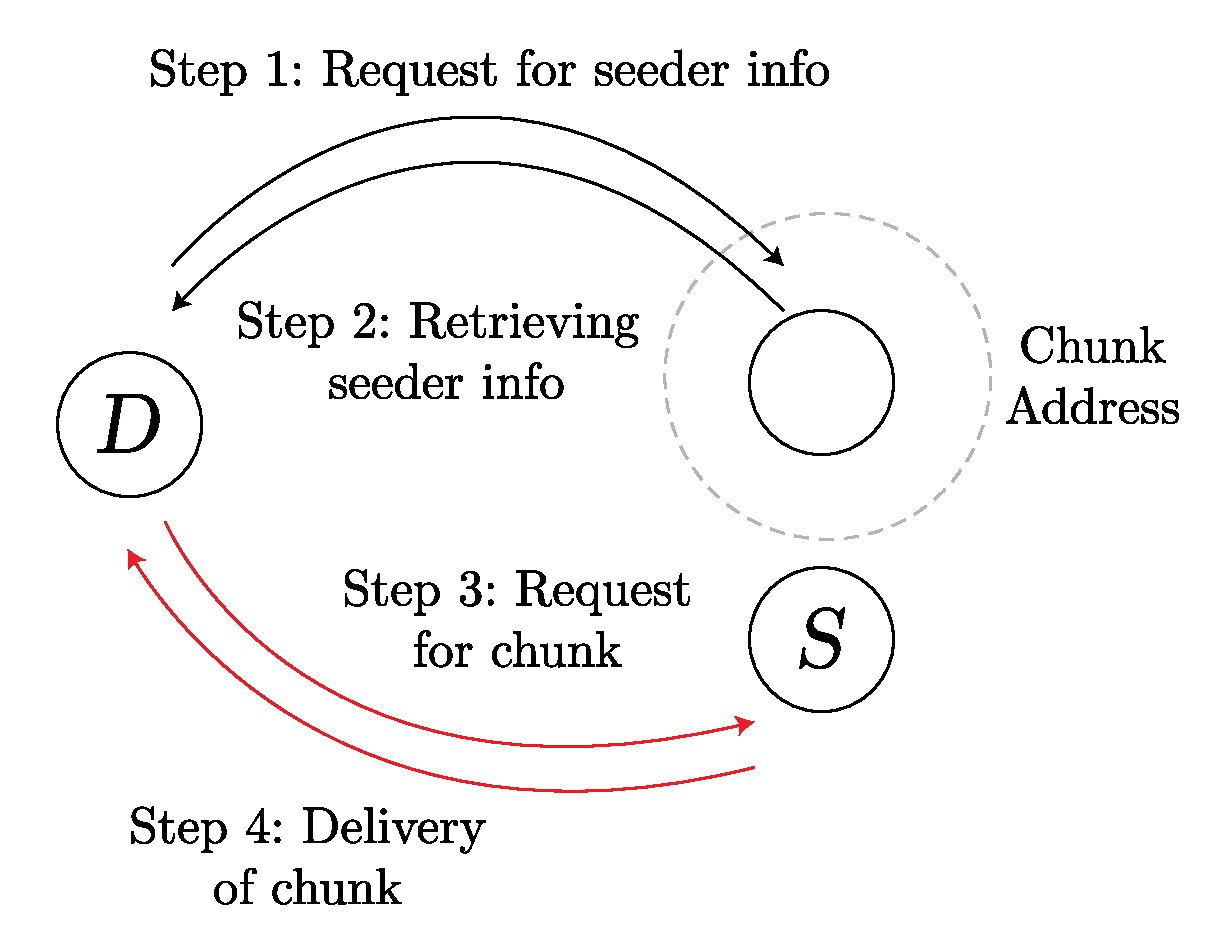
\includegraphics[width=0.7\textwidth]{fig/dht.pdf}
   \caption[Distributed hash tables (DHTs) \statusgreen]{Distributed hash tables (DHTs) used for storage:  node $D$ (downloader) uses Kademlia routing in step $1$ to query nodes in the neighbourhood of the chunk address to retrieve seeder info in step $2$. The seeder info is used to contact node $S$ (seeder) directly to request the chunk and deliver it in steps $3$ and $4$.}
   \label{fig:DHT}
\end{figure}

DHTs used for \gloss{distributed storage} typically associate content identifiers (as keys/addresses) with a changing list of seeders (as values) that can serve that content \cite{ipfs2014, crosby2007analysis}. However, the same structure can be used directly: in Swarm, it is not information about the location of content that is stored at the swarm node closest to the address, but the content itself (see figure \ref{fig:disc}). 


\begin{figure}[htbp]
   \centering
   \includegraphics[width=0.7\textwidth]{fig/disc.pdf}
   \caption[Swarm DISC: Distributed Immutable Store for Chunks \statusgreen]{Swarm DISC:  Distributed Immutable Store for Chunks. In step $1$, downloader node $D$ uses forwarding Kademlia routing to request the chunk from a storer node $S$ in the neighbourhood of the chunk address. In step $2$ the chunk is delivered along the same route using forwarding step just backwards.}
   \label{fig:disc}
\end{figure}

\subsubsection{Constraints}
The \gloss{DISC} storage model is opinionated about which nodes store what content and this implies the following restrictions: 

\begin{enumerate}
    \item \emph{fixed-size chunks} -- Load balancing of content is required among nodes and is realised by splitting content into equal sized units called \glossplural{chunk} (see \ref{sec:chunks}).
    \item \emph{syncing} -- There must be a process whereby chunks get to where they are supposed to be stored, no matter which node uploads them (see \ref{sec:push-syncing}).
    \item \emph{plausible deniability} -- Since nodes do not have a say in what they store, measures should be employed that serve as the basis of legal protection for node operators. They need to be able to plausibly deny knowing (or even being able to know) anything about the chunks' contents (see \ref{sec:chunk-encryption}).
    \item \emph{garbage collection} -- Since nodes commit to store anything close to them, there needs to be a strategy to select which chunks are kept and which are discarded in the presence of storage space constraints (see  \ref{spec:strategy:garbage-collection}). 
\end{enumerate}

\subsubsection{Chunks}\label{sec:chunks}

\glossupperplural{chunk} are the basic storage units used in Swarm's network layer. They are an association of an address with content. Since retrieval in Swarm (\ref{sec:retrieval}) assumes that chunks are stored with nodes close to their address, fair and equal \gloss{load balancing} requires that the addresses of chunks should also be uniformly distributed in the address space, and have their content limited and roughly uniform in size.  

When chunks are retrieved, the downloader must be able to verify the correctness of the content given the address. Such integrity translates to guaranteeing uniqueness of content associated with an address. In order to protect against frivolous network traffic, a third party \glossplural{forwarding node} should be able to verify the integrity of chunks using only local information available to the node.

The deterministic and collision free nature of addressing implies that chunks are unique as a key--value association: If there exists a chunk with an address, then no other valid chunk can have the same address; this assumption is crucial as it makes the chunk store \gloss{immutable}, i.e.\ there is no replace/update operation on chunks. Immutability is beneficial in the context of relaying chunks as nodes can negotiate information about the possession of chunks simply by checking their addresses. This plays an important role in the stream protocol (see \ref{sec:pull-syncing}) and justifies the DISC resolution as \emph{distributed immutable store for chunks}.

To sum up, chunk addressing needs to fulfill the following requirements:

\begin{enumerate}
    \item \emph{deterministic} -- To enable local validation.
    \item \emph{collision free} -- To provide integrity guarantee.
    \item \emph{uniformly distributed} -- To deliver load balancing.
\end{enumerate}

In the current version of Swarm, we support two types of chunk: \glossplural{content addressed chunk} and \glossplural{single owner chunk}. 

\subsection{Content addressed  chunks\statusgreen}\label{sec:content-addressed-chunks}

A \gloss{content addressed chunk} is not assumed to be a meaningful storage unit, i.e. they can be just blobs of arbitrary data resulting from splitting a larger data blob, a file. The methods by which files are disassembled into chunks when uploading and then reassembled from chunks when downloading are detailed in \ref{sec:datastructures}. The data size of a content addressed Swarm chunk is limited to 4 kilobytes. One of the desirable consequences of using this small chunk size is that concurrent retrieval is available even for relatively small files, reducing the latency of downloads. 

\begin{figure}[htbp]
   \centering
   
\includegraphics[width=\textwidth]{fig/content-addressed-chunk-3.pdf}
   \caption[Content addressed chunk\statusgreen]{Content addressed chunk. An at most 4KB payload with a 64-bit little endian encoded span prepended to it constitutes the chunk content. The BMT hash of the payload concatenated with the span then yields the content address.}
   \label{fig:content-addressed-chunk}
\end{figure}

\subsubsection{Binary Merkle tree hash}

The canonical content addressed chunk in Swarm is called a \gloss{binary Merkle tree chunk} (\gloss{BMT chunk}).
The address of BMT chunks is calculated using the \gloss{binary Merkle tree hash} algorithm (\gloss{BMT hash}) described in \ref{spec:format:bmt}. The base hash used in \gloss{BMT} is Keccak256, properties of which such as uniformity, irreversibility and collision resistance all carry over to the \gloss{BMT hash} algorithm. As a result of uniformity, a random set of chunked content will generate addresses evenly spread in the address space, i.e.\ imposing storage requirements balanced among nodes.


\begin{figure}[htbp]
   \centering
   \resizebox{1\textwidth}{!}{
   \input{fig/bmthash.tex}}
   \caption[BMT: Binary Merkle Tree hash used as chunk hash in Swarm \statusgreen]{BMT (Binary Merkle Tree) chunk hash in Swarm: the 1337 bytes of chunk data is segmented into 32 byte segments. Zero padding is used to fill up the rest up to 4 kilobytes. Pairs of segments are hashed together using Keccak256 to build up the binary tree. On level 8, the binary Merkle root is prepended with the 8 byte span and hashed to yield the BMT chunk hash.}
   \label{fig:BMT}
\end{figure}

The BMT chunk address is the hash of the 8 byte span and the root hash of a \gloss{binary Merkle tree} (\gloss{BMT}) built on the 32-byte segments of the underlying data (see figure \ref{fig:BMT}). If the chunk content is less than 4k, the hash is calculated as if the chunk was padded with all zeros up to 4096 bytes.

This structure allows for compact \gloss{inclusion proofs} with a 32-byte resolution. An inclusion proof is a proof that one string is a substring of another string, for instance, that a string is included in a chunk. Inclusion proofs are defined on a data segment of a particular index, see figure \ref{fig:chunk-inclusion}. Such Merkle proofs are also used as proof of custody when storer nodes provide evidence that they possess a chunk (see \ref{sec:postage-lottery}). Together with the Swarm file hash (see \ref{sec:files} and \ref{spec:format:files}), it allows for logarithmic inclusion proofs for files, i.e.,\ proof that a string is found to be part of a file.


\begin{figure}[htbp]
\centering
\includegraphics[width=\textwidth]{fig/inclusion-proof.pdf}
\caption[Compact segment inclusion proofs for chunks \statusgreen]{Compact segment inclusion proofs for chunks. Assume we need proof for segment 26 of a chunk (yellow). The orange hashes of the BMT are the sister nodes on the path from the data segment up to the root and constitute what needs to be part of a proof. When these are provided together with the root hash and the segment index, the proof can be verified. The side on which proof item $i$ needs to be applied depends on the $i$-th bit (starting from least significant) of the binary representation of the index. Finally the span is prepended and the resulting hash should match the chunk root hash.}
\label{fig:chunk-inclusion}
\end{figure}


\subsection{Single-owner chunks\statusgreen}\label{sec:single-owner-chunks}

With \glossplural{single owner chunk}, a user can assign arbitrary data to an address and attest chunk integrity with their digital signature. The address is calculated as the hash of an \gloss{identifier} and an \gloss{owner}. The chunk content is presented in a  structure composed of the identifier, the \gloss{payload} and a signature attesting to the association of identifier and payload (see figure \ref{fig:single-owner-chunks}).

\begin{itemize}
    \item \emph{content}: 
\begin{itemize}
    \item \emph{identifier} -- 32 bytes arbitrary identifier, 
    \item \emph{signature} -- 65 bytes $\langle r,s,v \rangle$ representation of an EC signature (32+32+1 bytes),
    \item \emph{span} -- 8 byte little endian binary of uint64 chunk span,
    \item \emph{payload} -- max 4096 bytes of regular chunk data.
\end{itemize}
    \item \emph{address} -- Keccak256 hash of identifier + owner account.
\end{itemize}

\begin{figure}[htbp]
   \centering
   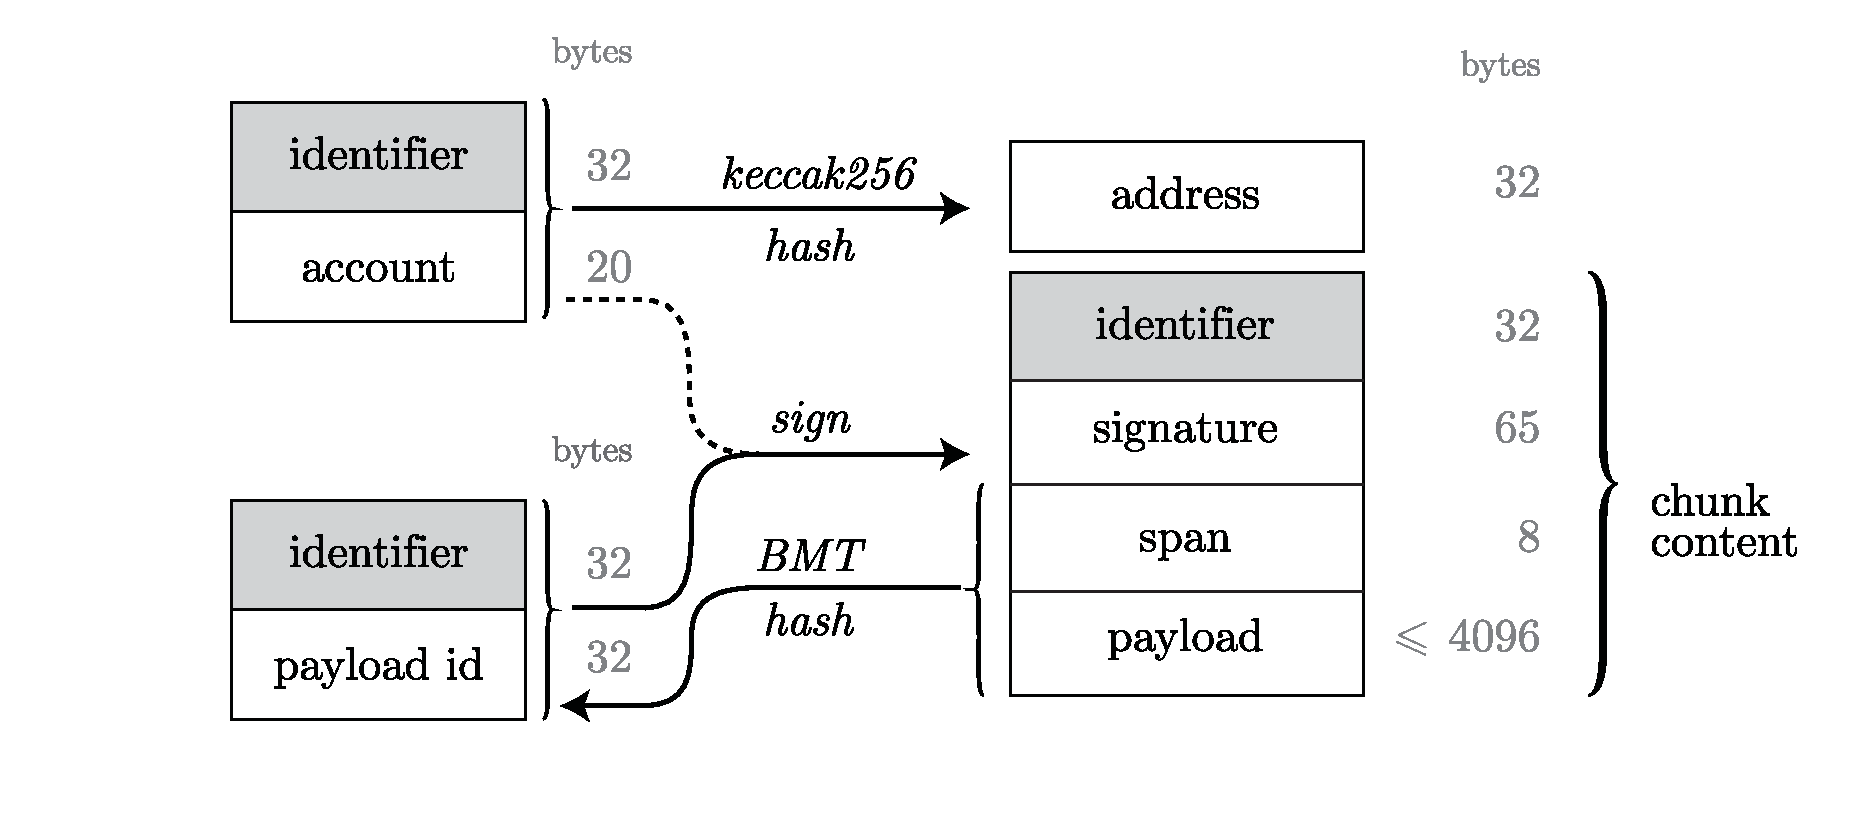
\includegraphics[width=\textwidth]{fig/single-owner-chunk.pdf}
   \caption[Single-owner chunk\statusgreen]{Single-owner chunk. The chunk content is composed of headers followed by an at most 4KB payload. The last header field is the 8 byte span prepended just like in content addressed chunks. The first two header fields provide single owner attestation of integrity: an identifier and a signature signing off on the identifier and the BMT hash of span and payload. The address is the hash of the id and the signer account.}
   \label{fig:single-owner-chunks}
\end{figure}

Validity of a \gloss{single owner chunk} is checked with the following process:

\begin{enumerate}
    \item Deserialise the chunk content into fields for identifier, signature and payload.
    \item Construct the expected plain text composed of the identifier and the \gloss{BMT hash} of the payload.
    \item Recover the owner's address from the signature using the plain text.
    \item Check the hash of the identifier and the owner (expected address) against the chunk address.
\end{enumerate}

Single-owner chunks offer a virtual partitioning of part of the address space into subspaces associated with the single owner. Checking their validity is actually an authentication verifying that the owner has write access to the address with the correct identifier.

As suggested by the span and the length of the payload, a single owner chunk can encapsulate a regular content addressed chunk. Anyone can simply reassign a regular chunk to an address in their subspace designated by the identifier (see also \ref{sec:notification-requests}).


It should be noted that the notion of integrity is somewhat weaker for single owner chunks than in the case of content addressed chunks: After all, it is, in principle, possible to assign and sign any payload to an identifier. Nonetheless, given the fact that the chunk can only be created by a single owner (of the private key that the signature requires), it is reasonable to expect uniqueness guarantees because we hope the node will want to comply with application protocols to get the desired result. However, if the owner of the private key signs two different payloads with the same identifier and uploads both chunks to Swarm, the behaviour of the network is unpredictable. Measures can be taken to mitigate this in layer (3) and are discussed later in detail in \ref{sec:feed-integrity}.

With two types of chunk, integrity is linked to collision free hash digests, derived from either a single owner and an arbitrary identifier attested by a signature or directly from the content. This justifies the resolution of the DISC acronym as \emph{data integrity through signing or content address}.

\subsection{Chunk encryption\statusgreen}\label{sec:chunk-encryption}

Chunks should be encrypted by default. Beyond client needs for confidentiality, encryption has two further important roles. (1) Obfuscation of chunk content by encryption provides a degree of \gloss{plausible deniability}; using it across the board makes this defense stronger. (2) The ability to choose arbitrary encryption keys together with the property of uniform distribution offer predictable ways of \gloss{mining chunks}, i.e.,\ generating an encrypted variant of the same content so that the resulting chunk address satisfies certain constraints, e.g. is closer to or farther away from a particular address. This is an important property used in (1) price arbitrage (see \ref{sec:pricing}) and (2) efficient use of postage stamps (see \ref{sec:postage-stamps}).


\begin{figure}[htbp]
    \centering
    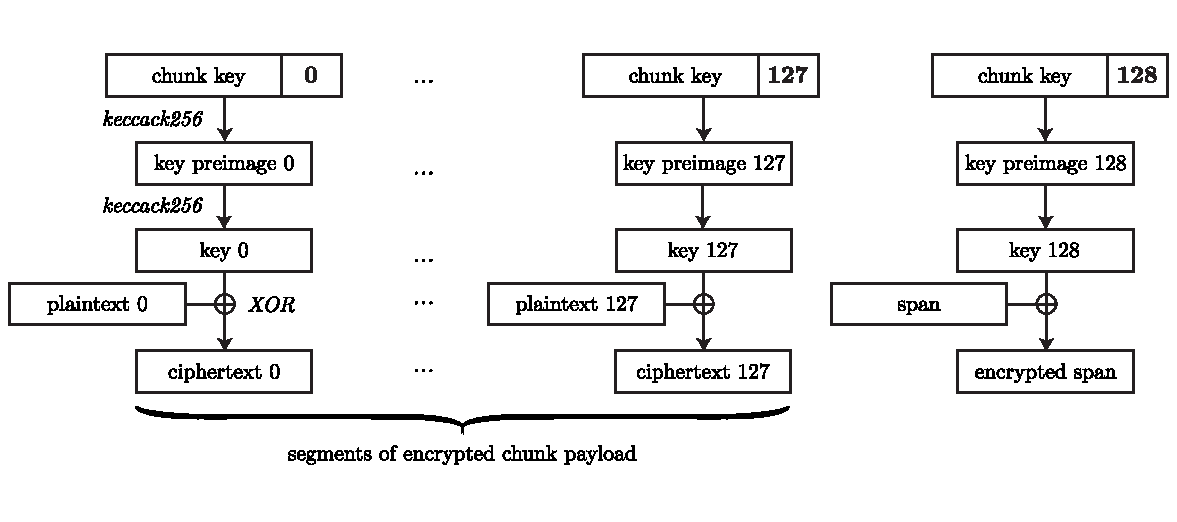
\includegraphics[width=\textwidth]{fig/chunk-encryption.pdf}
    \caption[Chunk encryption in Swarm \statusgreen]{Chunk encryption in Swarm. Symmetric encryption with a modified counter-mode block cipher. The plaintext input is the content padded with random bytes to 4 kilobytes. The span bytes are also encrypted as if they were continuations of the payload.}
    \label{fig:chunk-encryption}
\end{figure}


Chunk encryption (see figure \ref{fig:chunk-encryption}) is formally specified in \ref{spec:format:encryption}. Chunks shorter than 4 kilobytes are padded with random bytes (generated from the chunk encryption seed). The full chunk plaintext is encrypted and decrypted using a XOR-based block cipher seeded with the corresponding symmetric key. In order not to increase the attack surface by introducing additional cryptographic primitives, the block cipher of choice is using Keccak256 in counter mode, i.e. hashing together the key with a counter for each consecutive segment of 32 bytes. In order to allow selective disclosure of individual segments being part of an encrypted file, yet leak no information about the rest of the file, we add an additional step of hashing to derive the encryption key for a segment in the chunk. This scheme is easy and cheap to implement in the \gloss{EVM}, lending itself to use in smart contracts containing the plaintext of encrypted Swarm content. 

The prepended metadata encoding the chunk span is also encrypted as if it was a continuation of the chunk, i.e. with counter 128. Encrypted chunk content is hashed using the \gloss{BMT hash} digest just as unencrypted ones are. The fact that a chunk is encrypted may be guessed from the \gloss{span value}, but apart from this, in the network layer, encrypted chunks behave in exactly the same way as unencrypted ones.

\glossupperplural{single owner chunk} can also be encrypted, which simply means that they wrap an encrypted regular chunk. Therefore, their payload and span reflect the chunk content encryption described above, the hash signed with the identifier is the \gloss{BMT hash} of the encrypted span and payload, i.e. the same as that of the wrapped chunk.

\subsection{Redundancy by replication\statusgreen}\label{sec:redundancy-by-local-replication}

It is important to have a resilient means of requesting data. To achieve this Swarm implements the approach of defence in depth. In the case that a request fails due to a problem with forwarding, one can retry with another peer or, to guard against these occurrences, a node can start concurrent \glossplural{retrieve request} right away. However, such fallback options are not available if all the single last node that stores the chunk drop out from the network. Therefore, redundancy is of major importance to ensure data availability. If the closest node is the only storer of the requested data and it drops out of the network, then there is no way to retrieve the content. This basic scenario is handled by ensuring each set of \gloss{nearest neighbours} hold replicas of each chunk that is closest to any one of them, duplicating the storage of chunks and therefore providing data redundancy. 

\subsubsection{Size of nearest neighbourhoods}

If the Kademlia connectivity is defined over storer nodes, then in a network with Kademlia topology there exists a depth $d$ such that (1) each \gloss{proximity order bin} less than $d$ contains at least $k$ storer peers, and (2) all \glossplural{storer node} with \gloss{proximity order} $d$ or higher are actually connected peers. In order to ensure data redundancy, we can add to this definition a criterion that (3) the nearest neighbourhood defined by $d$ must contain at least $r$ peers.

Let us define \gloss{neighbourhood size} $\mathit{NHS}_x(d)$  as the cardinality of the neighbourhood defined by depth $d$ of node $x$. 
Then, a node has Kademlia connectivity with redundancy factor $r$ if there exists a depth $d$ such that (1) each proximity order bin less than $d$ contains at least $k$ storer peers ($k$ is the bin density parameter see \ref{sec:bindensity}), and (2) all storer nodes with proximity order $d$ or higher are actually connected peers, and (3) $\mathit{NHS}_x(d)\geq r$.

We can then take the highest depth $d'$ such that (1) and (2) are satisfied. Such a $d$ is guaranteed to exist and the \glossupper{hive protocol} is always able to bootstrap it. As we decrease $d'$, the amount of different neighbourhood grow proportionally, so for any redundancy parameter not greater than the network size $r\leq N=\mathit{NHS}_x(0)$, there will be a highest $0<d_r\leq d'$ such that $\mathit{NHS}_x(d_r)\geq r$. Therefore, \gloss{redundant Kademlia connectivity} is always achievable. 



For a particular redundancy, the area of the fully connected neighbourhood defines an \gloss{area of responsibility}. The proximity order boundary of the area of responsibility defines a \gloss{radius of responsibility} for the node. A storer node is said to be \emph{responsible} for (storing) a chunk if the chunk address falls within the node's radius of responsibility.

It is already instructive at this point to show neighbourhoods and how they are structured, see figure \ref{fig:nearest-neighbours}. 

\begin{figure}[htbp]
   \centering
   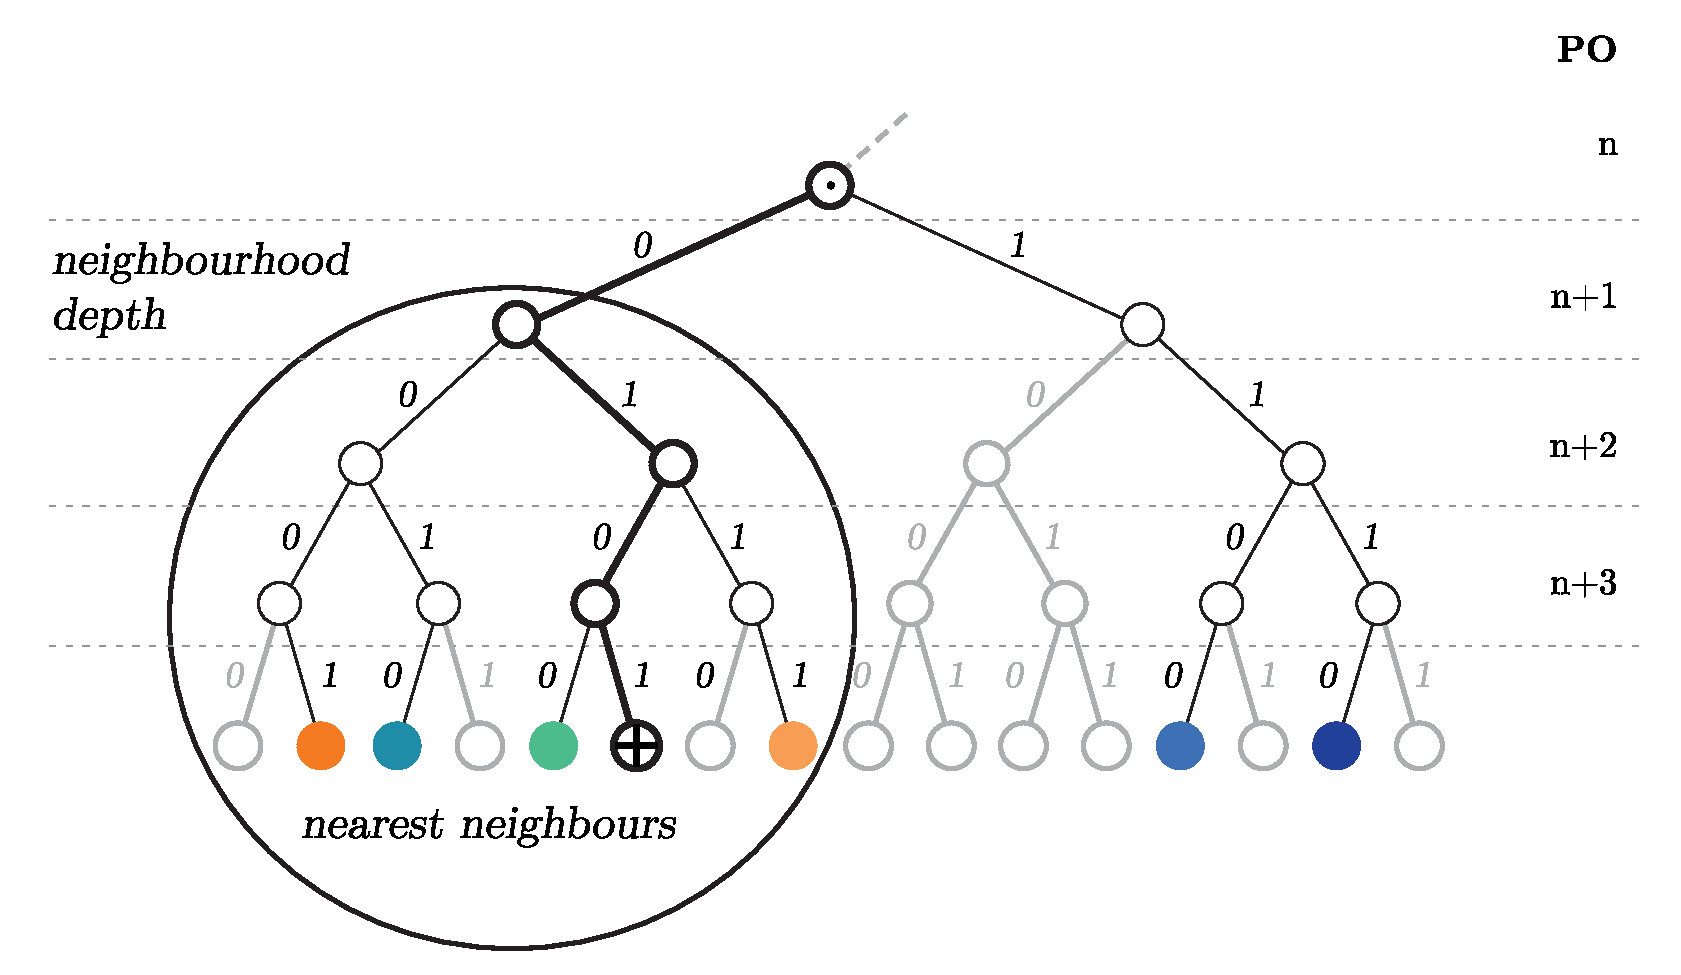
\includegraphics[width=\textwidth]{fig/nearest-neighbours-2.pdf}\\
   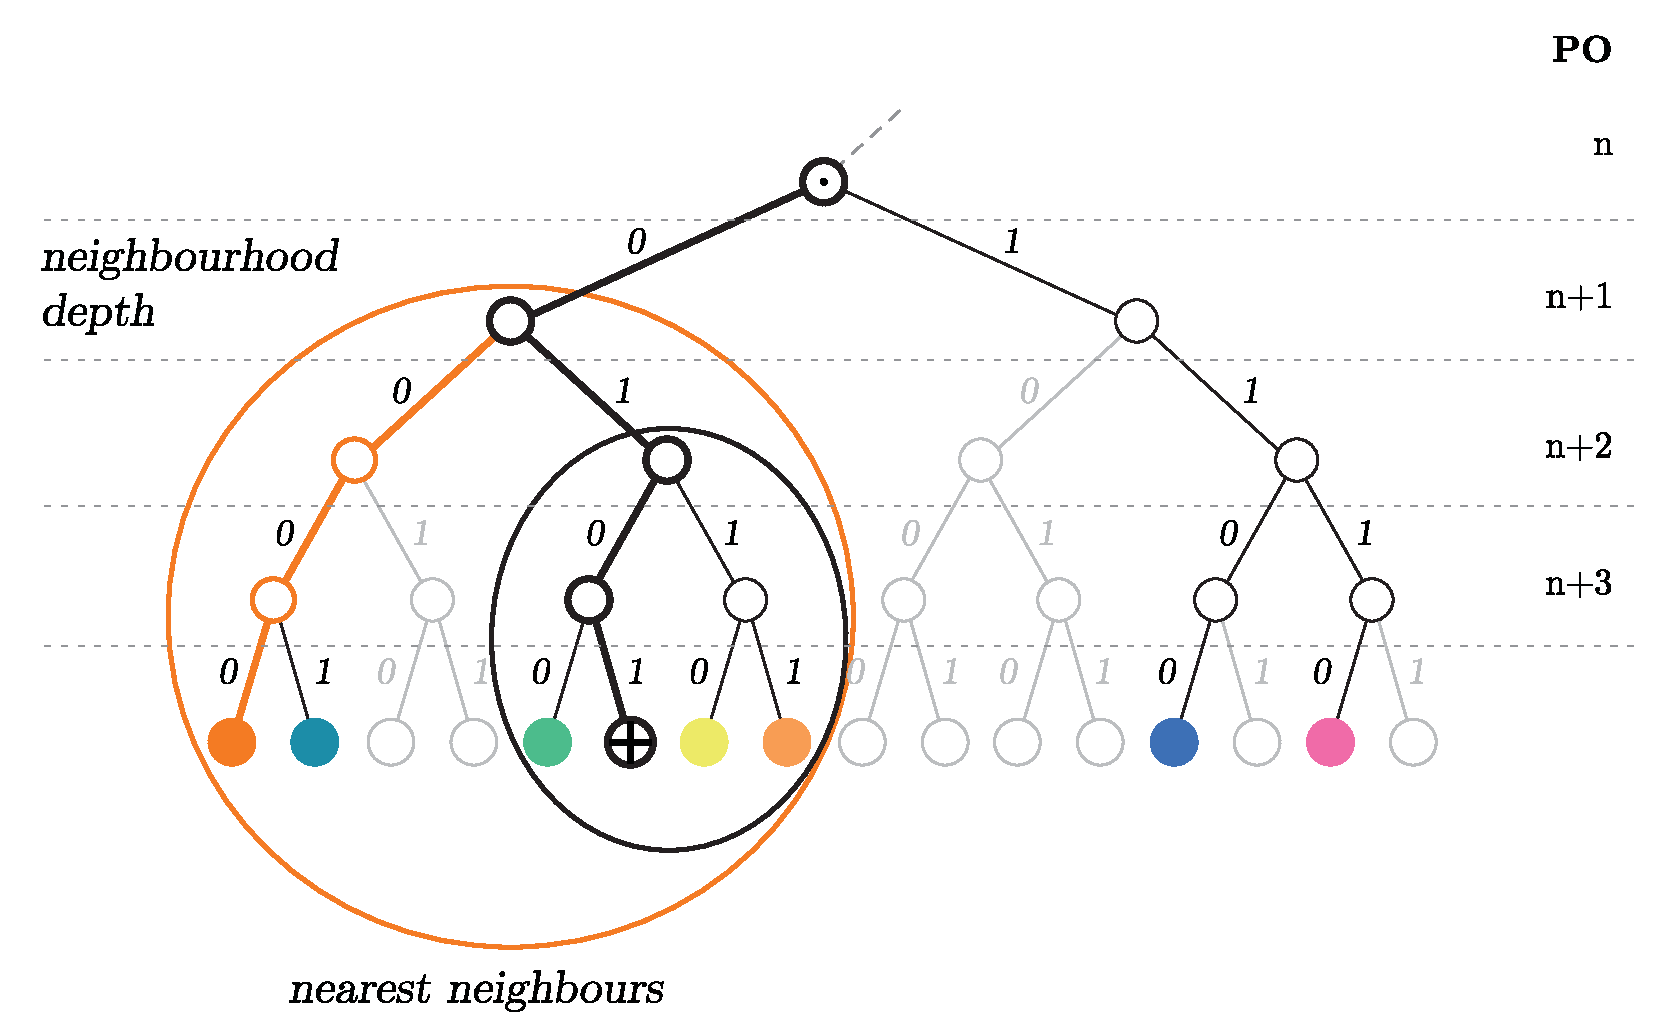
\includegraphics[width=\textwidth]{fig/asymmetric-nodes2.pdf}
   \caption[Nearest neighbours \statusgreen]{Nearest neighbours. \textbf{Top}: Each PO defines a neighbourhood, the neighbourhood depth of the node (black circle) is defined as the highest PO such that the neighbourhood has at least R=4 peers (redundancy parameter) and all shallower bins are non-empty. \textbf{Bottom}: An asymmetric neighbourhood. Nearest neighbours of the orange node include the black node but not the other way round.}
   \label{fig:nearest-neighbours}
\end{figure}


\subsubsection{Redundant retrievability}

A chunk is said to have \gloss{redundant retrievability} with degree $r$ if it is retrievable and would remain so even after any $r$ nodes responsible for it leave the network. The naive approach presented so far requiring the single closest node to keep the content can be interpreted as degree zero retrievability. If nodes in their area of responsibility fully replicate their content (see \ref{sec:pull-syncing}), then every chunk in the Swarm DISC is redundantly retrievable with degree $r$. Let us take the node $x$ that is closest to a chunk $c$. Since it has Kademlia connectivity with redundancy $r$, there are $r+1$ nodes responsible for the chunk in a neighbourhood fully connected and replicating content. After $r$ responsible nodes drop out, there is just one node remaining which still has the chunk. However, if Kademlia connectivity is maintained as the $r$ nodes leave, this node will continue to be accessible by any other node in the network and therefore the chunk is still retrievable. Now, for the network to ensure all chunks will remain redundantly retrievable with degree $r$, the nodes comprising the new neighbourhood formed due to the reorganising of the network must respond by re-syncing their content to satisfy the protocol's replication criteria. This is called the guarantee of \gloss{eventual consistency}.

\subsubsection{Resource constraints}

Let us assume then that (1) the forwarding strategy that relays requests along \glossplural{stable node} and (2) the storage strategy that each node in the nearest neighbourhood (of $r$ storer nodes) stores all chunks the address of which fall within their radius of responsibility. As long as these assumptions hold, each chunk is retrievable even if $r$ storer nodes drop offline simultaneously. As for (2), we still need to assume that every node in the nearest neighbour set can store each chunk. Realistically, however, all nodes have resource limitations. With time, the overall amount of distinct chunks ever uploaded to Swarm will increase indefinitely. Unless the total storage capacity steadily increases, we should expect that the nodes in Swarm are able to store only a subset of chunks. Some nodes will reach the limit of their storage capacity and therefore face the decision whether to stop accepting new chunks via syncing or to make space by deleting some of their existing chunks. 

The process that purges chunks from their local storage is called \gloss{garbage collection}. The process that dictates which chunks are chosen for garbage collection is called the \gloss{garbage collection strategy} (see  \ref{spec:strategy:garbage-collection}). For a profit-maximizing node, it holds that it is always best to garbage-collect the chunks that are predicted to be the least profitable in the future and, in order to maximize profit, it is desired for a node to get this prediction right (see \ref{sec:postage-stamps}). So, in order to factor in these capacity constraints, we will introduce the notion of \gloss{chunk value} and modify our definitions using the minimum value constraint:

In Swarm's DISC, at all times there is a chunk value $v$ such that every chunk with a value greater than $v$ is both retrievable and eventually (after syncing) redundantly retrievable with degree $r$. 

This value ideally corresponds to the relative importance of preserving the chunk that uploaders need to indicate. In order for storer nodes to respect it, the value should also align with the profitability of chunk and is therefore expressed in the pricing of uploads (see \ref{sec:capacity-pressure}).

% \subsection{}\label{sec:}

\section{Push and pull: chunk retrieval and syncing\statusgreen}\label{sec:push-and-pull}
\green{}
In this section, we demonstrate how chunks actually move around in the network: How they are pushed to the storer nodes in the neighbourhood they belong to when they are uploaded, as well as how they are pulled from the storer nodes when they are downloaded.

\subsection{Retrieval\statusgreen}\label{sec:retrieval}

In a distributed chunk store, we say that a chunk is an \gloss{accessible chunk} if a message is routable between the requester and the node that is closest to the chunk. Sending a retrieve request message to the chunk address will reach this node.  Because of \gloss{eventual consistency}, the node closest to the chunk address will store the chunk. Therefore, in a \gloss{DISC} distributed chunk store with healthy Kademlia topology all chunks are always accessible for every node.

\subsubsection{Chunk delivery}

For retrieval, accessibility needs to be complemented with a process to have the content delivered back to the requesting node, preferably using only the chunk address. There are at least three alternative ways to achieve this (see figure \ref{fig:chunk-delivery}):

\begin{enumerate}
    \item \gloss{direct delivery} -- The chunk delivery is sent via a direct underlay connection. 
    \item \gloss{routed delivery} -- The chunk delivery is sent as message using routing.
    \item \gloss{backwarding} -- The chunk delivery response simply follows the route along which the request was forwarded, just backwards all the way to the originator.
\end{enumerate}


\begin{figure}[htbp]
   \centering
   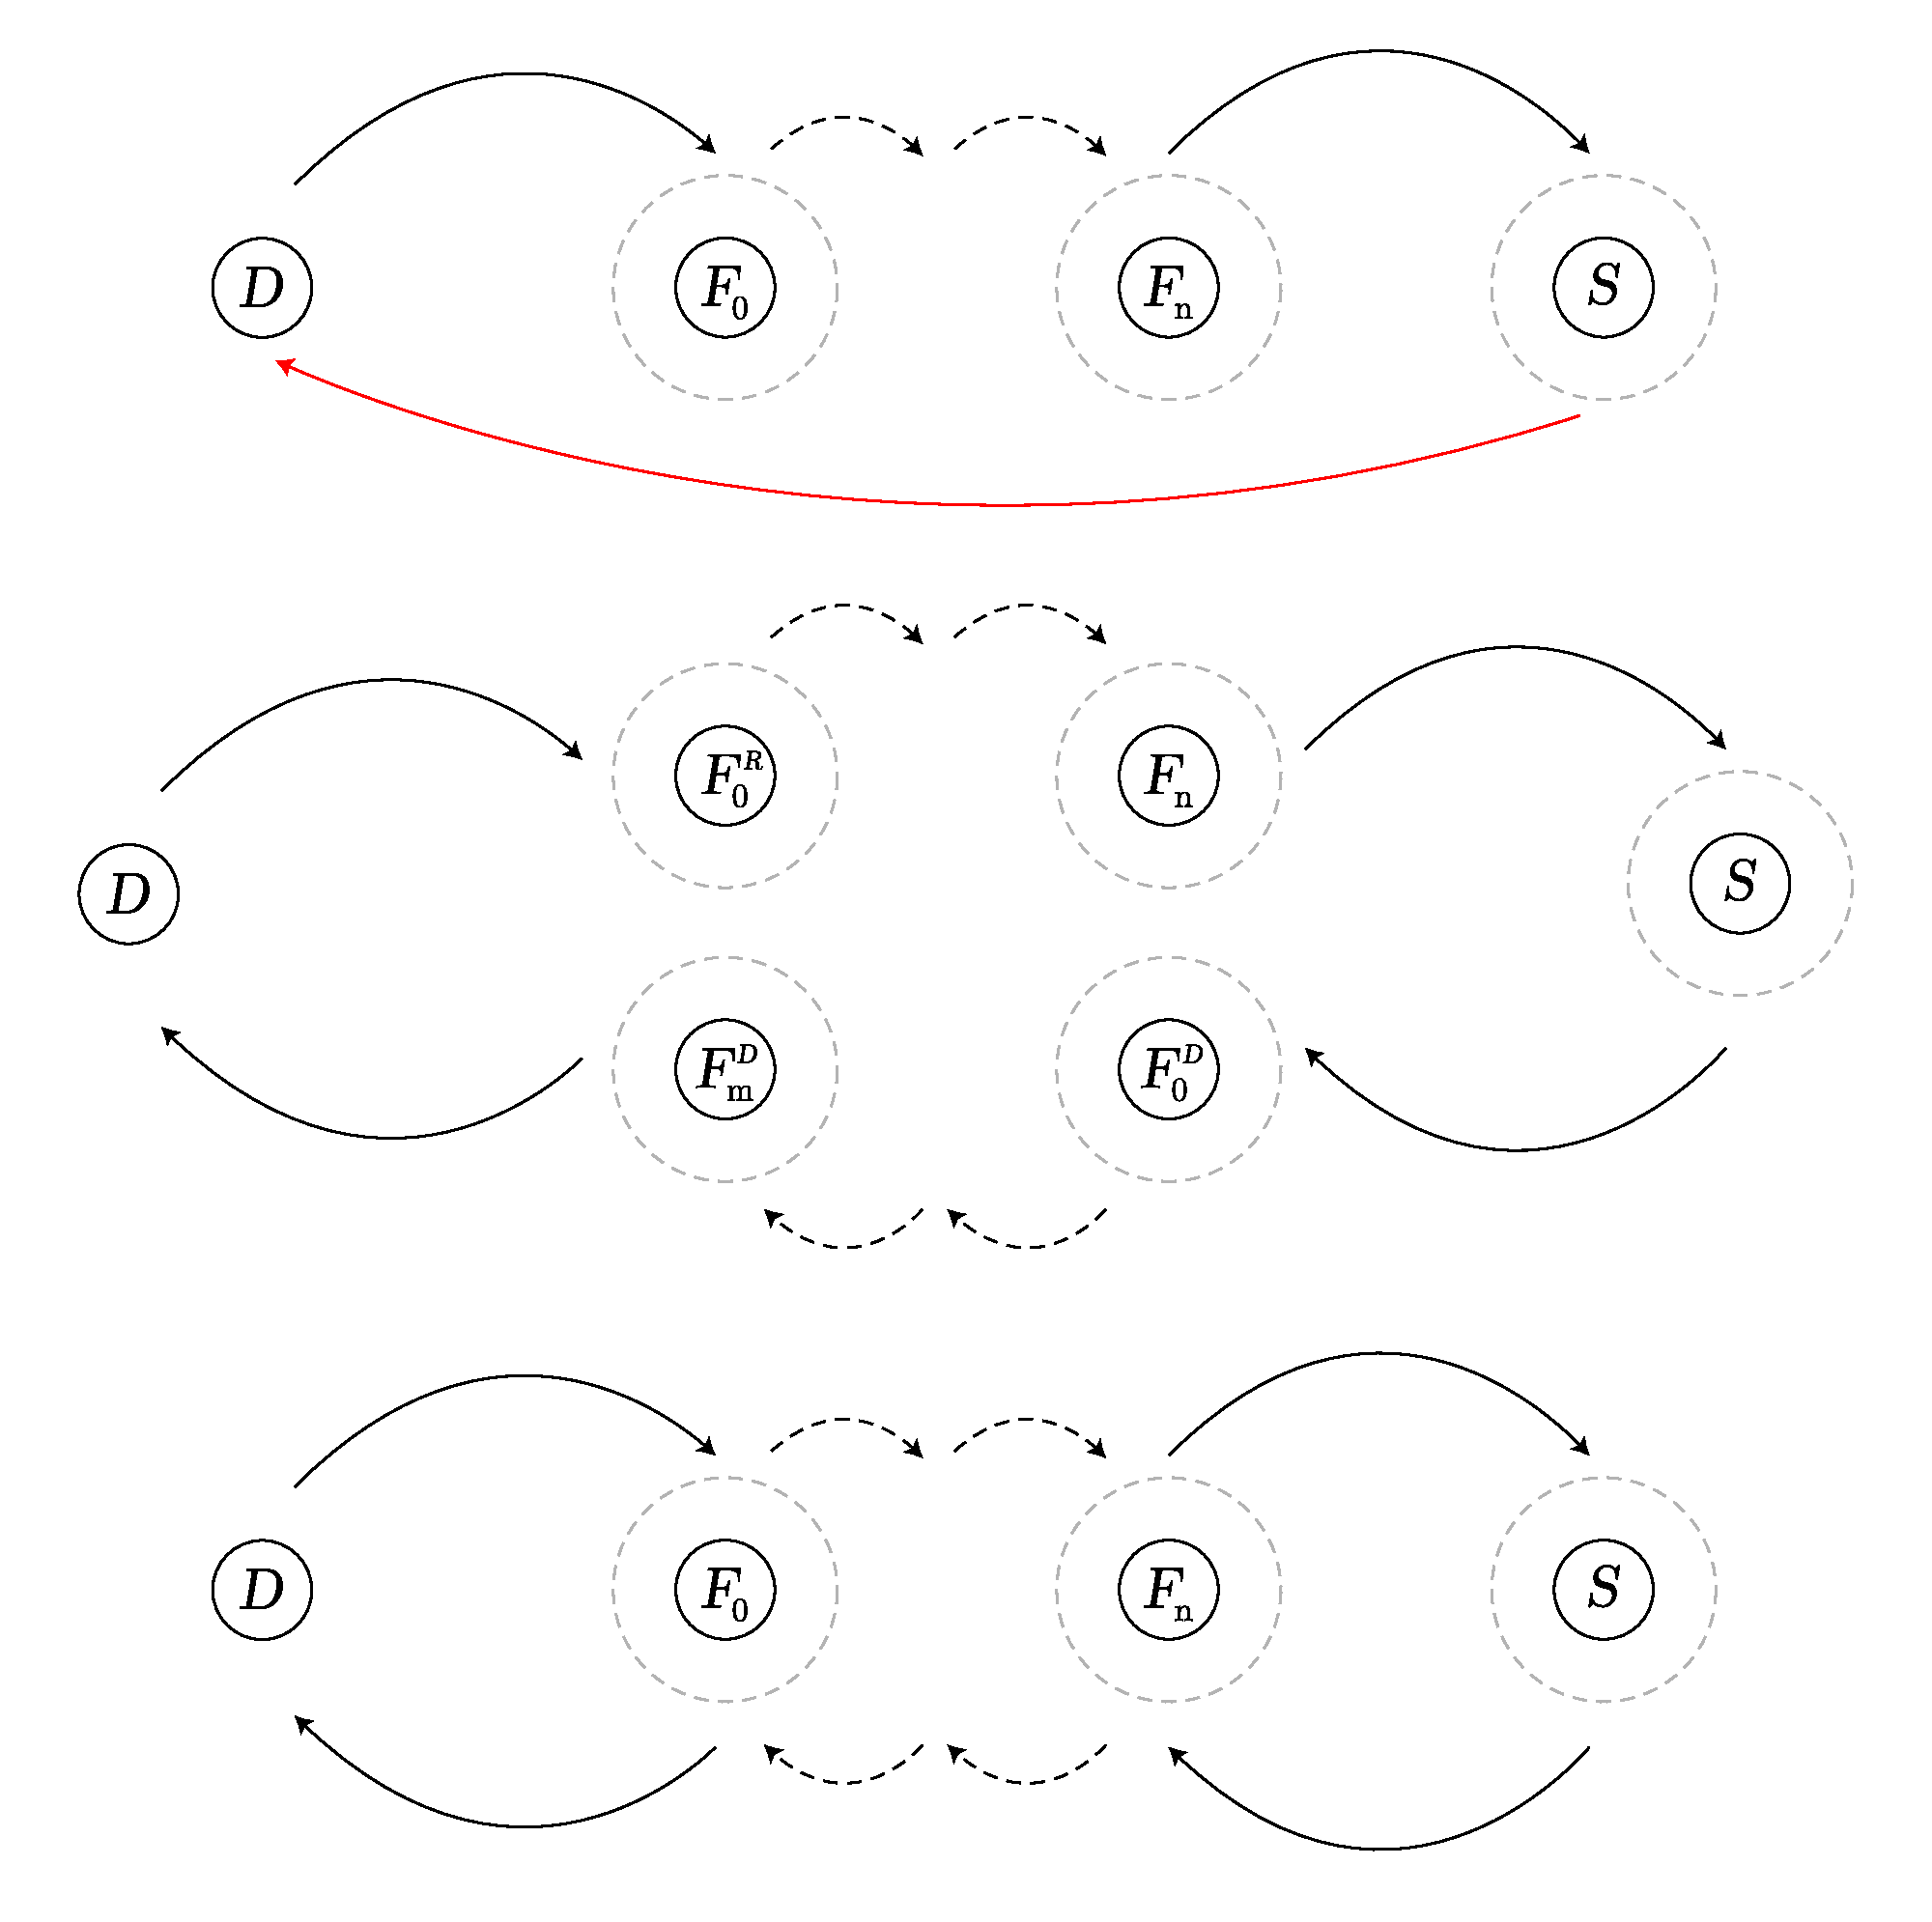
\includegraphics[width=\textwidth]{fig/chunk-delivery.pdf}
   \caption[Alternative ways to deliver chunks: direct, routed and backward \statusgreen]{Alternative ways to deliver chunks. \textbf{Top:} \emph{direct delivery}: via direct underlay connection. \textbf{Centre:} \emph{routed delivery}: chunk is sent using Kademlia routing. \textbf{Bottom:} \gloss{backwarding} re-uses the exact peers on the path of the request route to relay the delivery response.}
   \label{fig:chunk-delivery}
\end{figure}

Firstly, using the obvious direct delivery, the chunk is delivered in one step via a lower level network protocol. This requires an ad-hoc connection with the associated improvement in latency traded off for worsened security of privacy.%
%
\footnote{Beeline delivery has some merit, i.e. bandwidth saving and better latency, so we do not completely rule out the possibility of implementing it. 
}
Secondly, using routed delivery, a chunk is delivered back to its requestor using ad-hoc routing as determined from the storer's perspective at the time of sending it. Whether direct or routed, allowing deliveries routed independently of the request route presupposes that the requestor's address is (at least partially) known by the storer and routing nodes and as a consequence, these methods leak information identifying the requestor. However, with forwarding--backwarding Kademlia this is not necessary: The storer node responds back to their requesting peer with the delivery while intermediate \glossplural{forwarding node} remember which of their peers requested what chunk. When the chunk is delivered, they pass it on back to their immediate requestor, and so on until it eventually arrives at the node that originally requested it. In other words, the chunk delivery response simply follows the request route back to the originator (see figure \ref{fig:request-response}).  Since it is the reverse of the forwarding, we can playfully call this \gloss{backwarding}. Swarm uses this option, which makes it possible to disclose no requestor identification in any form, and thus Swarm implements completely \gloss{anonymous retrieval}. 

\begin{figure}[htbp]
   \centering
   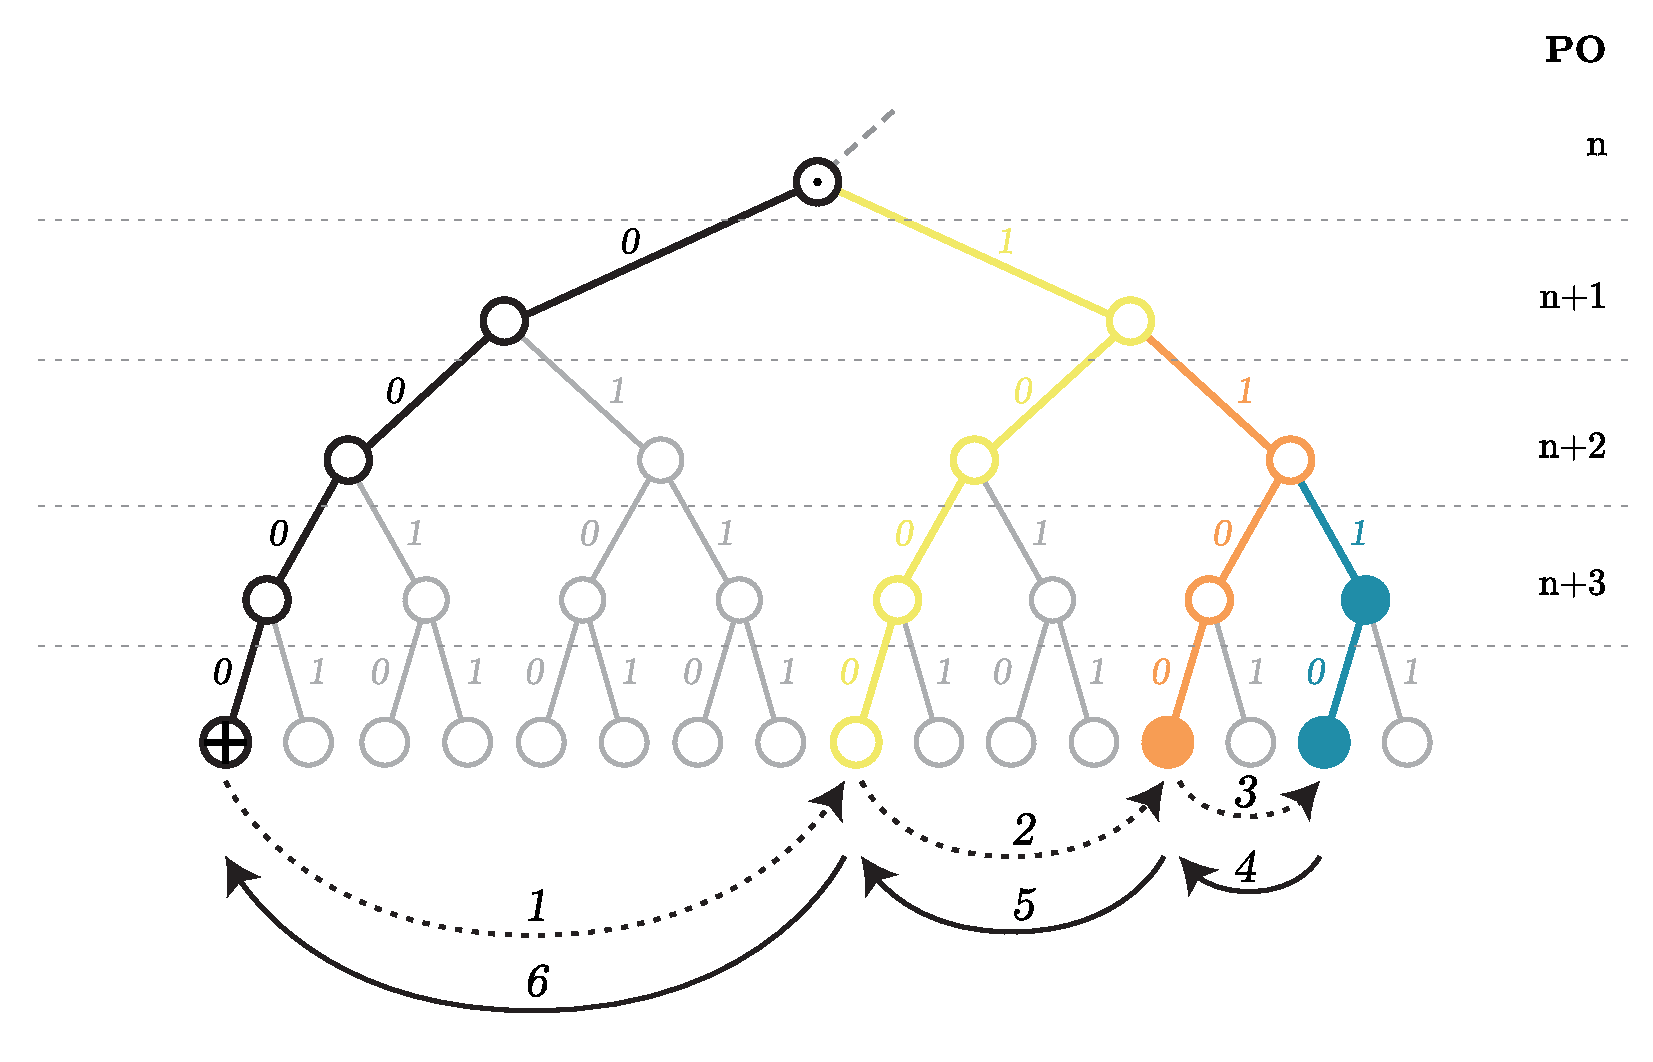
\includegraphics[width=\textwidth]{fig/request-response-forwarding.pdf}
   \caption[Backwarding: a pattern for anonymous request-response round-trips in forwarding Kademlia \statusgreen]{Backwarding: pattern for anonymous request--response round-trips in forwarding Kademlia. Here a node with overlay address $...0000...$ sending a request to target $....1111...$ to which the closest online node is $...1110...$ The leading ellipsis represents the prefix shared by the requestor and target and has a length of $n$ bits, the trailing ellipsis represents part of the address that is not relevant for routing as at that depth nodes are already unique. The request uses the usual Kademlia forwarding, but the relaying nodes on the way remember the peer a request came from so that when the response arrives, they can \emph{backward} it (i.e.\ pass it back) along the same route.}
   \label{fig:request-response}
\end{figure}

Requestor anonymity by default in the retrieval protocol is a crucial feature that Swarm insists upon to ensure user privacy and censorship-resistant access.

\begin{figure}[htbp]
   \centering
   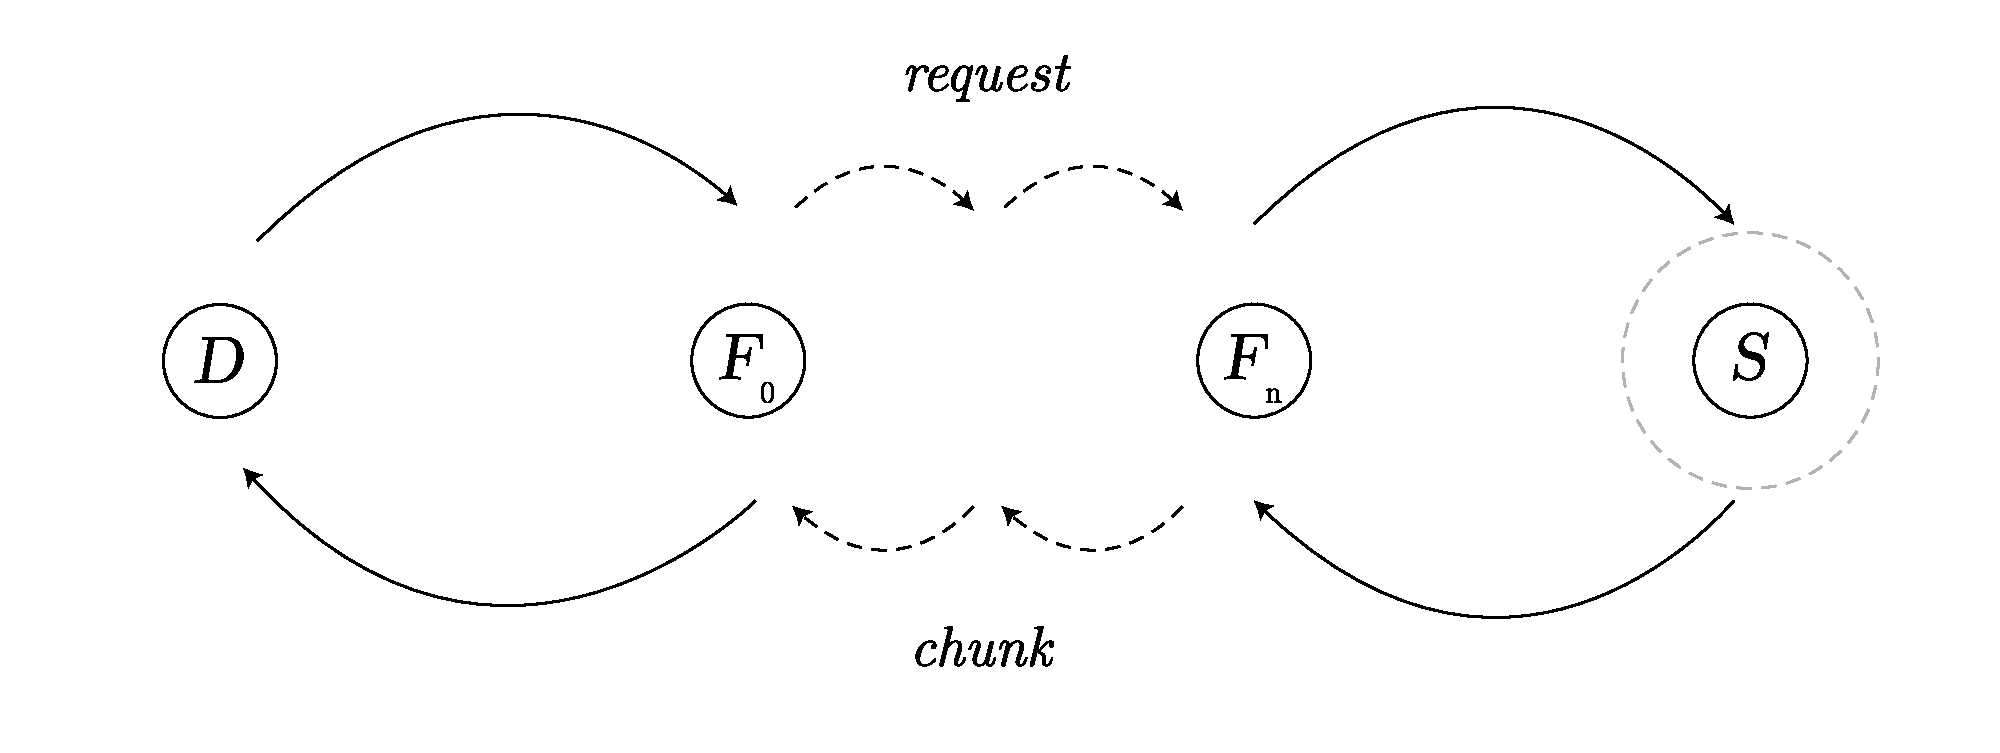
\includegraphics[width=\textwidth]{fig/retrieval.pdf}
   \caption[Retrieval \statusgreen]{Retrieval. Node $D$ (Downloader) sends a retrieve request to the chunk's address. Retrieval uses forwarding Kademlia, so the request is relayed via forwarding nodes $F_0$, ..., $F_n$ all the way to node $S$, the storer node closest to the chunk address. The chunk is then delivered by being passed back along the same route to the downloader.}
   \label{fig:retrieval}
\end{figure}

The generic solution of implementing retrieval by backwarding as depicted in figure \ref{fig:retrieval} has further benefits relating to spam protection, scaling and incentivisation, which are now discussed in the remainder of this section.

\subsubsection{Protection against unsolicited chunks}

In order to remember requests, the \gloss{forwarding node} needs to create a resource for which it bears some cost (it takes up space in memory). The requests that are not followed by a corresponding delivery should eventually be garbage collected, so there needs to be a defined time period during which they are active. Downstream peers also need to be informed about the timeout of this request. This makes sense since the originator of the request will want to attach a time to live duration to the request to indicate how long it will wait for a response.  

Sending unsolicited chunks is an offence as it can lead to \gloss{denial of service (DoS)}. By remembering a request, nodes are able to recognise unsolicited chunk deliveries and penalise the peers sending them. Chunks that are delivered after the request expires will be treated as unsolicited. Since there may be some discrepancy assessing the expiry time between nodes, there needs to be some tolerance for unsolicited chunk deliveries, but if they go above a particular (but still small) percentage of requests forwarded, the offending peer is disconnected and blacklisted. Such local sanctions are the easiest and simplest way to incentivise adherence to the protocol (see \ref{sec:sanctions}). 

\subsubsection{Rerequesting}

There is the potential for a large proportion of Swarm nodes to not be always stably online. Such a high churn situation would be problematic if we used the naive strategy of forwarding requests to any one closer node: If a node on the path were to go offline before delivery is completed, then the request-response round trip is broken, effectively rendering the chunk requested not retrievable. Commitment to pay for a chunk is considered void if the connection to the requested peer is dropped, so there is no harm in re-requesting the chunk from another node (see \ref{spec:strategy:forwarding}).


\subsubsection{Timeout vs not found}

Note that in Swarm there is no explicit negative response for chunks not being found. In principle, the node that is closest to the retrieved address can tell that there is no chunk at this address and could issue a "not found" response, however this is not desirable for the following reason. While the closest node to a chunk can verify that a chunk is indeed not at the place in the network where it is supposed to be, all nodes further away from the chunk cannot credibly conclude this as they cannot verify it first-hand and all positive evidence about the chunk's retrievability obtained later is retrospectively plausibly deniable. 

All in all, as long as delivery has the potential to create earnings for the storer, the best strategy is to keep a pending request open until it times out and be prepared in case the chunk should appear. There are several ways the chunk could arrive after the request: (1) syncing from existing peers (2) appearance of a new node or (3) if a request precedes upload, e.g. the requestor has already "subscribed" to a single owner address (see \ref{sec:messaging}) to decrease latency of retrieval. This is conceptually different from the usual server-client based architectures where it makes sense to expect a resource to be either on the host server or not. 
 

\subsubsection{Opportunistic caching}

Using the backwarding for chunk delivery responses to retrieve requests also enables \gloss{opportunistic caching}, where a \gloss{forwarding node} receives a chunk and the chunk is then saved in case it will be requested again. This mechanism is crucial in ensuring that Swarm scales the storage and distribution of popular content automatically (see \ref{sec:caching}).

\subsubsection{Incentives}

So far, we have shown that by using the retrieval protocol and maintaining Kademlia connectivity, nodes in the network are capable of retrieving chunks. However, since forwarding is expending a scarce resource (bandwidth), without providing the ability to account for this bandwidth use, network reliability will be contingent on the proportion of freeriding and altruism. To address this, in section \ref{sec:incentivisation}, we will outline a system of economic incentives that align with the desired behaviour of nodes in the network. When these profit maximising strategies are employed by node operators, they give rise to emergent behaviour that is beneficial for users of the network as a whole.
 
\subsection{Push syncing\statusgreen}\label{sec:push-syncing}
 
In the previous sections, we presented how a network of nodes maintaining a Kademlia overlay topology can be used as a distributed chunk store and how Forwarding Kademlia routing can be used to define a protocol for retrieving chunks.
When discussing retrieval, we assumed that chunks are located with the node whose address is closest to theirs. This section describes the protocol responsible for realising this assumption: ensuring delivery of the chunk to its prescribed storer after it has been uploaded to any arbitrary node.

This network protocol, called \gloss{push syncing}, is analogous to chunk retrieval: First, a chunk is relayed to the node closest to the chunk address via the same route as a retrieval request would be, and then in response a \gloss{statement of custody receipt} is passed back along the same path (see figure \ref{fig:push-syncing}). The statement of custody sent back by the storer to the \gloss{uploader} indicates that the chunk has reached the neighbourhood from which it is then universally retrievable. By tracking these responses for each constituent chunk of an upload, uploaders can make sure that their upload is fully retrievable by any node in the network before sharing or publishing the address of their upload. Keeping this count of chunks push-synced and receipts received serves as the back-end for a \emph{progress bar} that can be displayed to the uploader to give feedback of the successful propagation of their data across the network (see \ref{sec:upload} and \ref{spec:api:tags}).


\begin{figure}[htbp]
   \centering
   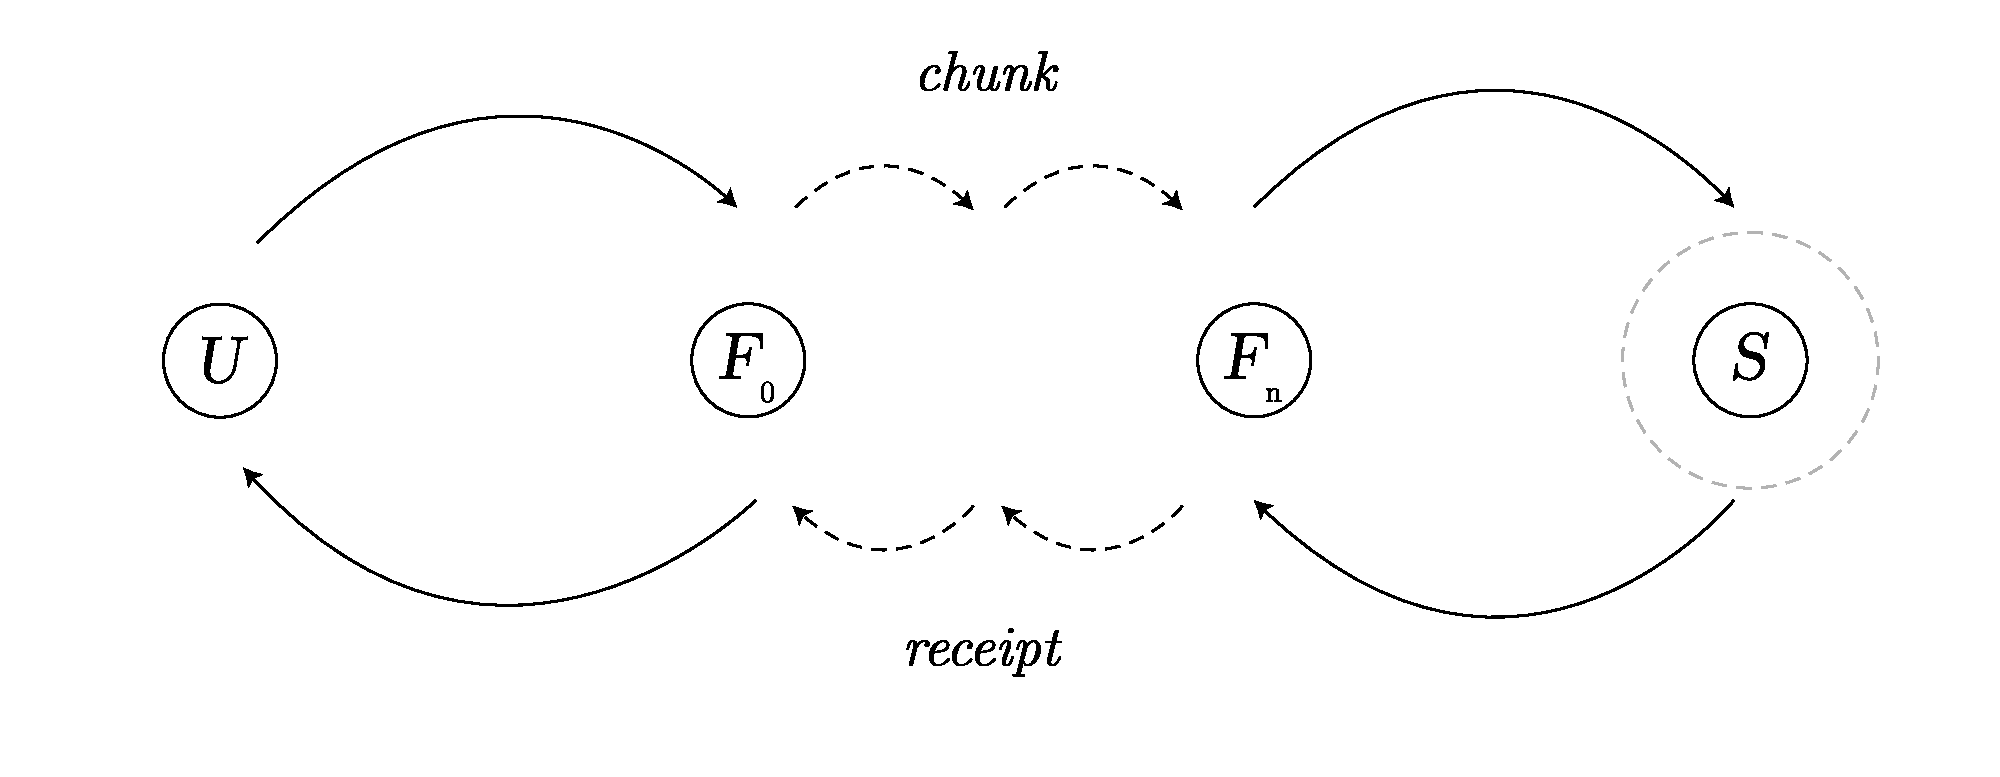
\includegraphics[width=\textwidth]{fig/push-sync.pdf}
   \caption[Push syncing \statusgreen]{Push syncing. Node $U$ (Uploader) push-syncs a chunk to the chunk's address. Push-sync uses forwarding, so the chunk is relayed via forwarding nodes $F_0$, ..., $F_n$ all the way to node $S$, the storer node closest to the chunk address (the arrows represent transfer of the chunk  via direct peer-to-peer connection). A statement of custody receipt signed by $S$ is then passed back along the same route as an acknowledgment to the uploader.}
   \label{fig:push-syncing}
\end{figure}

Statements of custody are signed by the nodes that claim to be the closest to the address. 
Similarly to downloaders in the retrieval protocol, the identity of uploaders can also remain hidden, hence forwarding Kademlia can implement \gloss{anonymous uploads}.

Another similarity is that in order to allow backwarding for responses, nodes should remember which peer sent a particular chunk. This record should persist for a short period while the statement of custody responses are expected. When this period ends, the record is removed. A statement of custody not matching a record is considered unsolicited and is allowed only up to a small percentage of all push-sync traffic with a peer. Going above this tolerance threshold is sanctioned with disconnection and blacklisting (see \ref{sec:sanctions}).

In this section we described how the logistics of chunk uploads can be organised with a network protocol using Forwarding Kademlia routing with response backwarding. However, this solution is not complete until it is secured with aligned incentives: The strategy to follow this protocol should be incentivised and DoS abuse should be disincentivised. These are discussed later in detail in \ref{sec:postage-stamps} and \ref{sec:push-sync-incentives}).

\subsection{Pull syncing\statusgreen}\label{sec:pull-syncing}

\glossupper{pull syncing} is the protocol that is responsible for the following two properties: 

\begin{itemize}
    \item \emph{eventual consistency} -- Syncing neighbourhoods as and when the topology changes due to churn or new nodes joining.
    \item \emph{maximum resource utilisation} -- Nodes can pull chunks from their peers to fill up their surplus storage.%
%
\footnote{Maximum storage utilisation may not be optimal in terms of the profitability of nodes. Put differently, storer nodes have an optimal storage capacity, based on how often content is requested from them. This means that in practice, profit-optimised maximum utilisation of storage capacity requires operators to run multiple node instances.}
\end{itemize}

Pull syncing is node centric as opposed to chunk centric, i.e. it makes sure that a node's storage is filled if needed, as well as syncing chunks within a neighbourhood. When two nodes are connected they will start syncing both ways so that on each peer connection there is bidirectional chunk traffic. The two directions of syncing are managed by distinct and independent \emph{streams} (see \ref{spec:protocol:pull-sync}). In the context of a stream, the consumer of the stream is called \gloss{downstream peer} or client, while the provider is called the \gloss{upstream peer} or server. 

When two nodes connect and engage in \gloss{chunk synchronisation}, the upstream peer offers all the chunks it stores locally in a data stream per proximity order bin. To receive chunks closer to the downstream peer than to the upstream peer, a downstream peer can subscribe to the chunk stream of the proximity order bin that the upstream peer belongs to in their Kademlia table. If the peer connection is within the nearest neighbour depth $d$, the client subscribes to all streams with proximity order bin $d$ or greater. As a result, peers eventually replicate all chunks belonging to their area of responsibility.

A pull syncing server's behaviour is referred to as being that of a \gloss{stream provider} in the stream protocol (see \ref{spec:protocol:pull-sync}). Nodes keep track of when they stored a chunk locally by indexing them with an ever increasing storage count, called the \gloss{bin ID}. For each proximity order bin, upstream peers offer to stream chunks in descending order of storage timestamp. As a result of syncing streams on each peer connection, a chunk can be synced to a downstream peer from multiple upstream peers. In order to save bandwidth by not sending data chunks to peers that already have them, the stream protocol implements a round-trip: Before sending chunks, the upstream peer offers a batch of chunks identified by their address, to which downstream responds with stating which chunks in the offered batch they actually need (see figure \ref{fig:pull-syncing}). Note that downstream peer decides whether they have the chunk based on the chunk address. Thus, this method critically relies on the chunk integrity assumption discussed in \ref{sec:chunks}.


\begin{figure}[htbp]
   \centering
   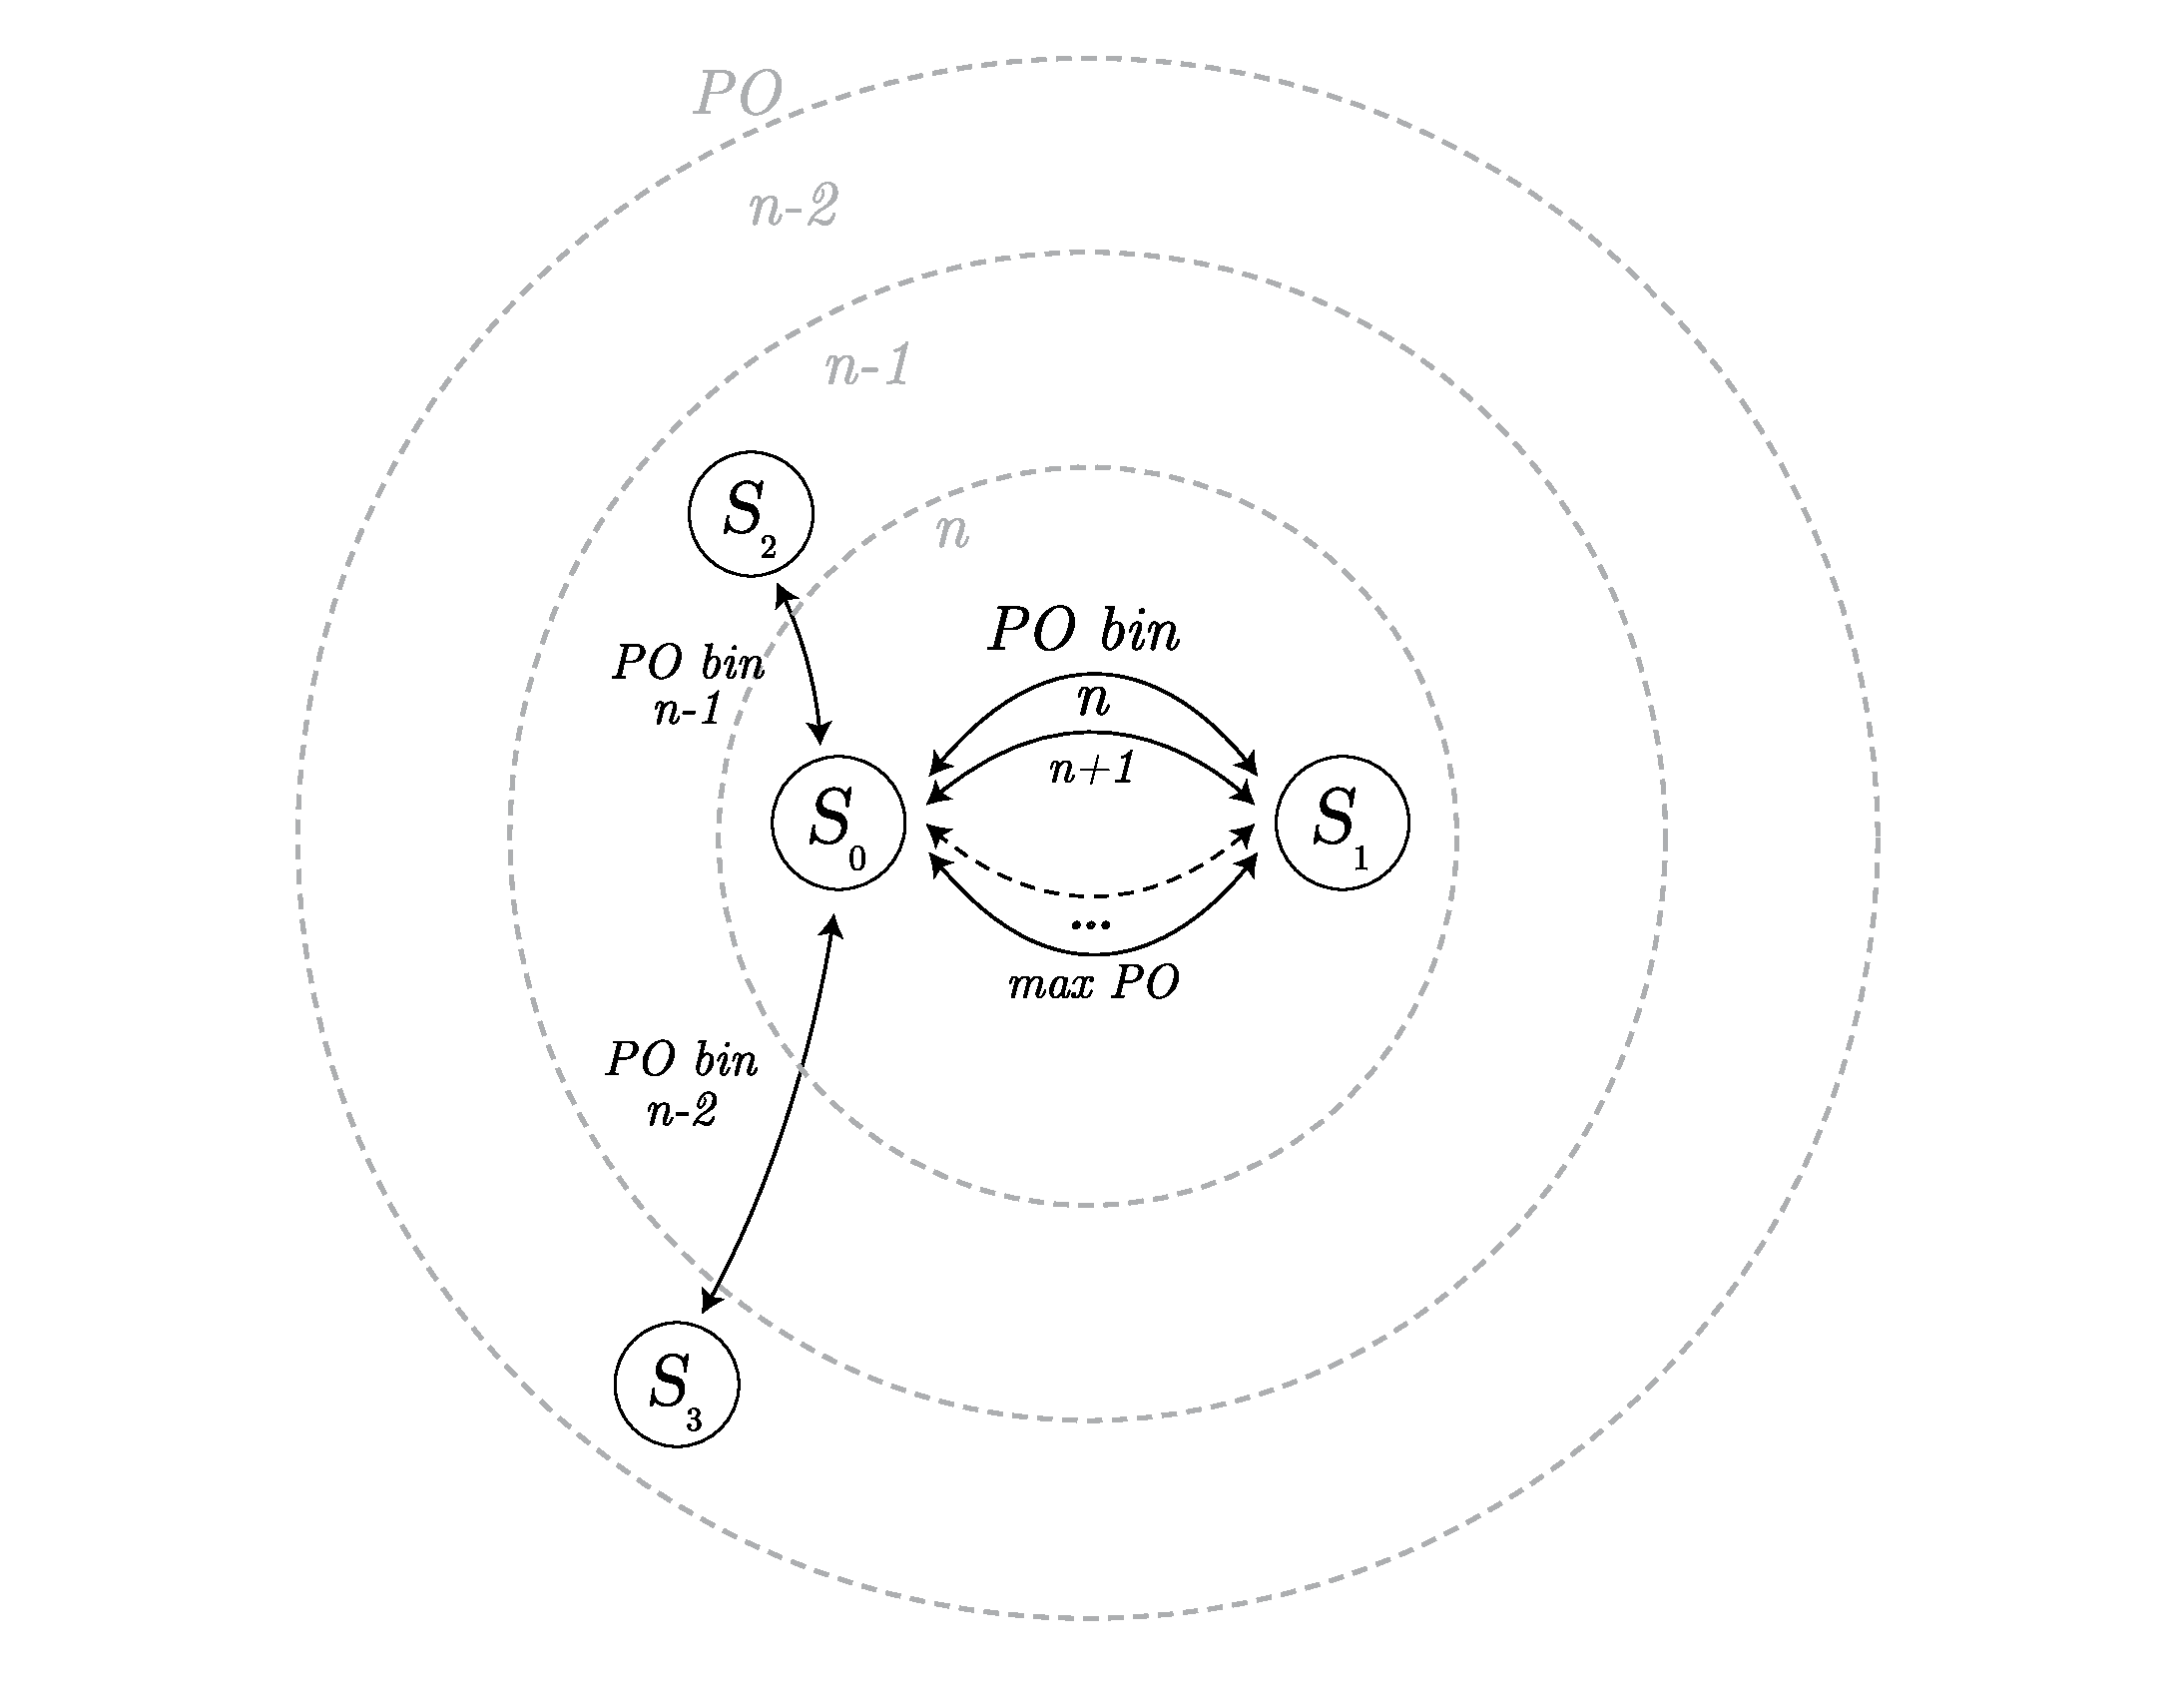
\includegraphics[width=\textwidth]{fig/pull-sync.pdf}
   \caption[Pull syncing \statusgreen]{Pull syncing. Nodes continuously synchronise their nearest neighbourhood. If they have free capacity they also pull sync chunks belonging to shallower bins from peers falling outside the neighbourhood depth.}
   \label{fig:pull-syncing}
\end{figure}

In the context of a peer connection, a client is said to be \emph{synced} if it has synced all the chunks of the upstream peer. Note that due to disk capacity limitations, nodes must impose a value cutoff and as such "all chunks" reads as shorthand for "all chunks having value greater than $v$" ($v$ is a constant ranking function, the origin of which is discussed later in \ref{sec:capacity-pressure}). In order for a node to promise they store all chunks with value greater than $v$, all its neighbours must have stored all chunks greater than value $v$. In other words, nodes syncing inherit the maximum such value from among their storer peers. 

If chunks are synced in the order they are stored, this may not result in the node always having the most profitable (most often requested) chunks. Thus it may be advisable to sync chunks starting with the most popular ones according to upstream peers and finish syncing when storage capacity is reached. In this way, a node's limited storage will be optimised. Syncing and garbage collection are discussed further in \ref{sec:postage-stamps} and \ref{sec:capacity-pressure} and a consolidated client strategy is specified in \ref{spec:strategy:pull-sync}.

To conclude this section, we show how the criteria of \gloss{eventual consistency} are met in a healthy Swarm. Chunks found in the local store of any node will become retrievable after being synced to their storers. This is because as long as those as peers in the network pull chunks closer to them than to the upstream peer, each chunk travels a route that would also qualify as valid a forwarding path in the push-sync protocol. If new nodes are added, and old nodes drop out, neighbourhoods change, but as long as local redundancy is high enough that churn can not render previously retrievable chunks non-retrievable, neighbourhoods eventually replicate their content and redundancy is restored. Consider the unlikely event that a whole new neighbourhood is formed and the nodes that originally held the content belonging to this neighbourhood end up outside of it and therefore those chunks are temporarily not available. Even in this scenario, as long as there is a chain of nodes running pull-syncing streams on the relevant bins, redundant retrievability is eventually restored.

\subsection{Light nodes\statusgreen}
\label{sec:light}

The concept of a \gloss{light node} refers to a special mode of operation necessitated by poor bandwidth environments, e.g. mobile devices on low throughput networks or devices allowing only transient or low-volume storage.

A node is said to be light by virtue of not participating fully in the usual protocols detailed in the previous sections, i.e. retrieval, push syncing or pull syncing. 

A node that has restricted bandwidth environment or in whatever way has limited capacity to maintain underlay connections is not expected to be able to forward messages conforming to the rules of Kademlia routing. This needs to be communicated to its peers so that they do not relay messages to it. 

As all protocols in Swarm are modular, a node may switch on or off any protocol independently (depending on capacity and earnings requirements). To give an example: a node that has no storage space available, but has spare bandwidth, may participate as a forwarding node only. Of course, while switching off protocols is technically feasible, a node must at all times take into account the fact that his peers expect a certain level of service if this is advertised and may not accept that some services are switched off and choose not to interact with that node. 

Since forwarding can earn revenue, these nodes may still be incentivised to accept retrieve requests. However, if the light node has Kademlia connectivity above proximity order bin $p$ (i.e. they  are connected to all storer nodes within their nearest neighbourhood of $r$ peers at depth $d$, and there is at least one peer in each of their proximity order bin from $p$ to $d$), they can advertise this and therefore participate in forwarding. 

When they want to retrieve or push chunks, if the chunk address falls into a proximity order bin where there are no peers, they can just pick a  peer in another bin. Though this may result in a spurious hop (where the proximity of the message  destination to the latest peer does not increase as a result of the relaying), the Kademlia assumption that routing can be completed in logarithmic steps still holds valid.

A node that is advertised as a storer/caching node is expected to store all chunks  above a certain value. In order to have consistency, they need to synchronise content in their area of responsibility which necessitates their running of the pull-sync protocol. This is also so with aspiring storer nodes, which come online with available storage and open up to pull-sync streams to fill their storage capacity. In the early stages of this, it does not make sense for a node to sync to other full storer nodes. However, it can still be useful for them to sync with other similar newcomer nodes, especially if storer nodes are maxing out on their bandwidth.

The crucial thing here is that for redundancy and hops to work, light nodes with   incomplete, unsaturated Kademlia tables should not be counted by other peers towards saturation.


\chapter{Incentives}\label{sec:incentivisation}
The Swarm network comprises many independent nodes, running software which implements the Swarm protocol (see chapter \ref{spec:protocol}). It is important to realize that, even though nodes run the same protocol, the emergent behavior of the network is not guaranteed by the protocol alone; as nodes are autonomous, they are essentially "free" to react in any way they desire to incoming messages of peers.
It is, however possible to make it profitable for a node to react in a way that is beneficial for the desired emergent behavior of the network, while making it costly to act in a way that is detrimental. Broadly speaking, this is achieved in Swarm by enabling a transfer of value from those nodes who are using the resources of the network (\glossplural{net user}) to those who are providing it (\glossplural{net provider}). 


\begin{figure}[htbp]
\centering
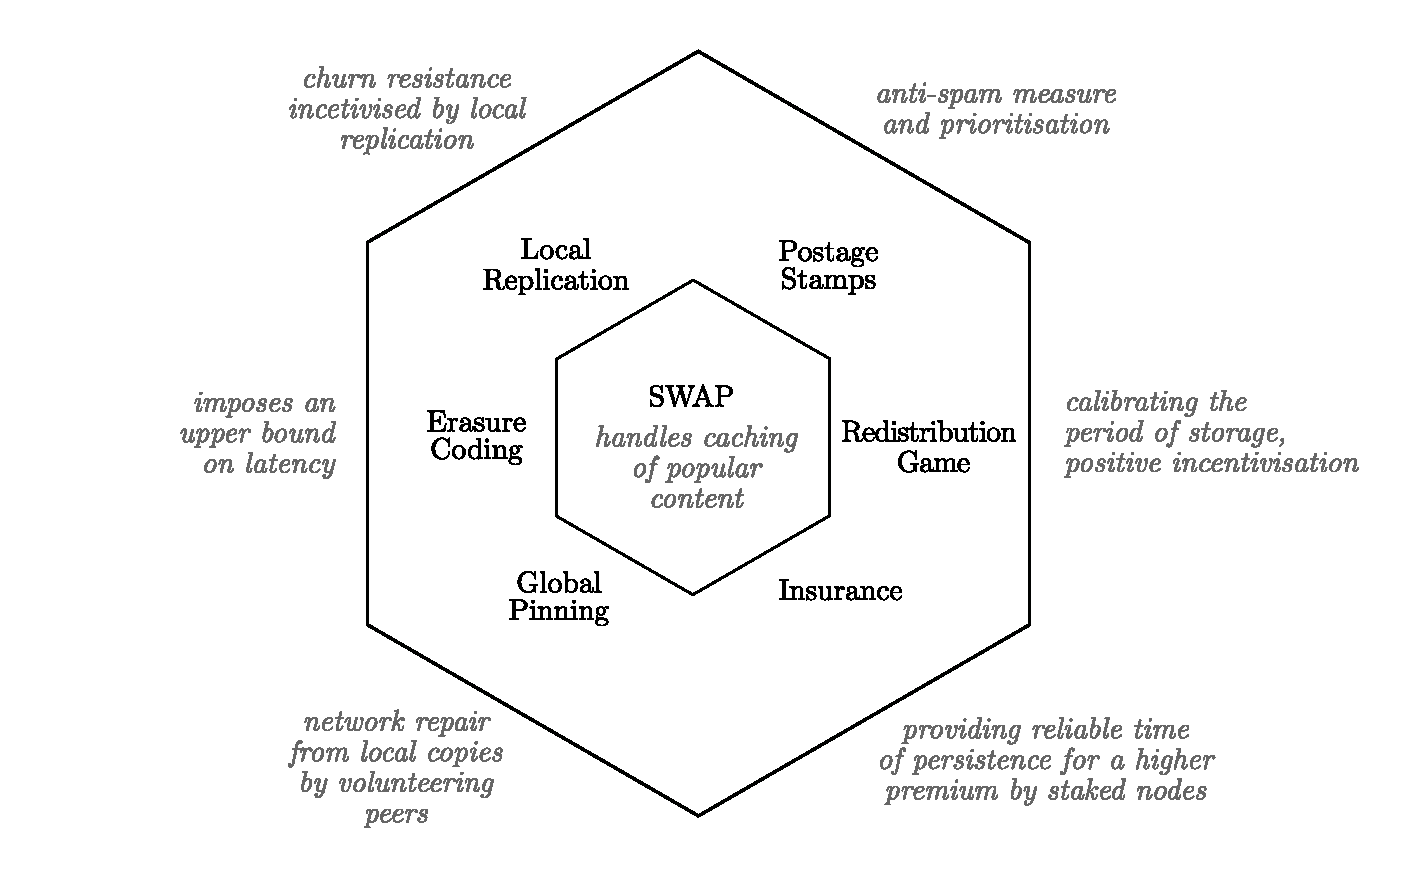
\includegraphics[width=\textwidth]{fig/incentive-design-3.pdf}
\caption[Incentive design \statusgreen]{Incentive design}
\label{fig:incentives}
\end{figure}

% The rest of this chapter is concerned with describing the desired emergent behaviour of the network (\ref{sec:emergent_behavior}), after which we describe the actions which incur costs and those that provide value (\ref{sec:cost_benefit}). Finally, we proceed by describing the incentive mechanisms which ensures that costs are borne as directly as possible by the initiator of the action, with benefits flowing to the nodes who provided the initiator with the expected outcome, ultimately facilitating the desired emergent behavior (see \ref{sec:incentive_mechanisms}).

% \section{Incentive design \statusred}
% \wip{foundational requirement + analysis} 
% \subsection{WIP Desired emergent behavior \statusred}\label{sec:emergent_behavior}
% \subsection{WIP Analysis on expected costs and benefits of actions \statusred}\label{sec:cost_benefit}
% \subsection{WIP Proposed incentive mechanisms \statusred}\label{sec:incentive_mechanisms}
% This section will constitute most of the sections which are already described below.


\section{Sharing bandwidth\statusgreen}

\green{}

\subsection{Incentives for serving and relaying\statusgreen}\label{sec:incentives-relaying}

\green{}

\subsubsection{Forwarding Kademlia and repeated dealings}

Retrieval of a chunk is ultimately initiated by someone accessing content and therefore, all costs related to this retrieval should be borne by them. While paid retrievals may not sound like a popular idea when today's web is "free", many of the problems with the current web stems from consumers' inability to share the costs of hosting and distribution with content publishers directly. In principle, the retrieval of a chunk can be perceived as a functional unit where the storer acts as a service provider and the requestor as consumer. As service is given by provider to consumer, compensation should be given by consumer to provider. Such a direct transaction would normally require that transactors are known to each other, so if we are to maintain the anonymity requirement on downloads, we must conceptualise compensation in a novel way. 

As we use Forwarding Kademlia, chunk retrieval subsumes a series of relaying actions performed by forwarding nodes. Since these are independent actors, it is already necessary to incentivise each act of relaying independently. Importantly, if only instances of relaying are what matters, then, irrespective of the details of accounting and compensation (see \ref{sec:accounting}), transactors are restricted to connected peers. Given the set of ever connected peers is a quasi-permanent set across sessions, this allows us to frame the interaction in the context of repeated dealings. Such a setting always creates extra incentive for the parties involved to play nice. It is reasonable to exercise preference for peers showing untainted historical record. Moreover, since the set of connected peers is logarithmic in the network size, any book-keeping or blockchain contract that the repeated interaction with a peer might necessitate is kept manageable, offering a scalable solution. Turning the argument around, we could say that keeping balances with a manageable number of peers, as well as the ambiguity of request origination are the very reasons for nodes to have limited connectivity, i.e., that they choose leaner Kademlia bins.

\subsubsection{Charging for backwarded response}

If accepting a retrieve request already constitutes revenue for forwarding nodes, i.e. an accounting event crediting the downstream peer is triggered before the response is delivered, then it creates a perverse incentive not to forward the requests. Conditioning the request revenue fulfilment on successful retrieval is the natural solution: The accounting event is triggered only when a requested chunk is delivered back to its requestor, see figure \ref{fig:retrieval-payment}.


\begin{figure}[htbp]
   \centering
   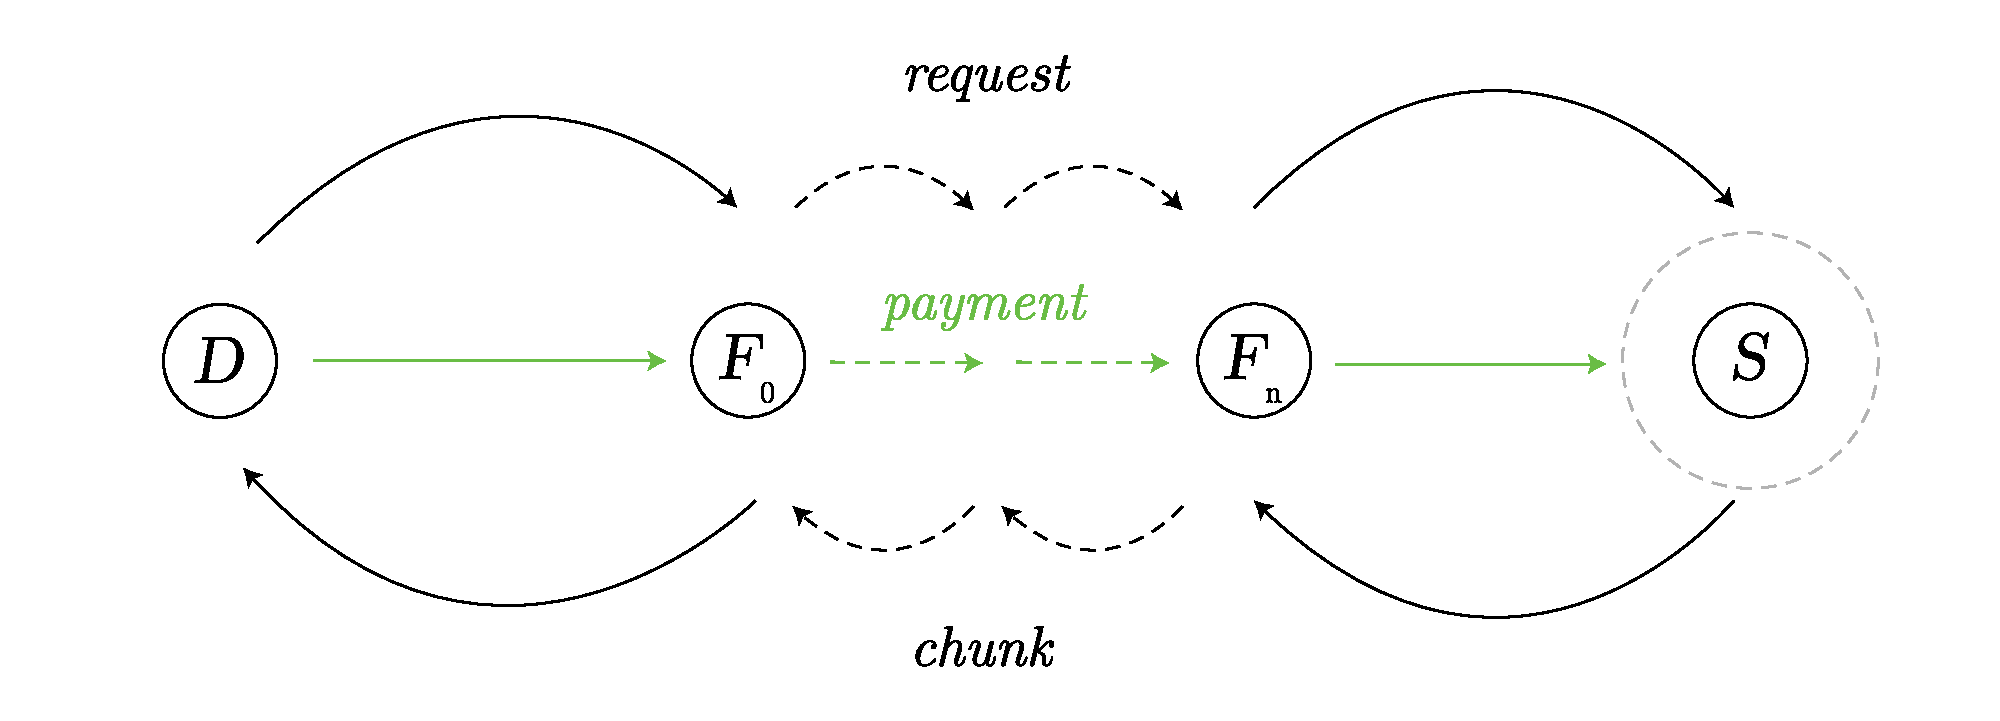
\includegraphics[width=\textwidth]{fig/retrieval-payment.pdf}
   \caption[Incentivising retrieval \statusgreen]{Incentivising retrieval. Node $D$ (Downloader) sends a retrieve request to the chunk's address. Retrieval uses forwarding, so the request is relayed via forwarding nodes $F_0$, ..., $F_n$ all the way to node $S$, the storer node closest to the chunk address. The chunk is delivered by being passed back along the same route to the downloader. Receiving the chunk response triggers an accounting event.}
   \label{fig:retrieval-payment}
\end{figure}

If, however, there is no cost to a request, then sending many illegitimate requests for non-existing chunks (random addresses) becomes possible. This is easily mitigated by imposing sanctions on peers that send too many requests for chunks that do not exist (see \ref{sec:sanctions}).

Once a node initiates (starts or forwards) a request, it commits to pay for that chunk if it is delivered within the defined \gloss{time to live} (\gloss{TTL}), therefore there is never an incentive to block timely deliveries when the chunk is passed back.  This commitment also dissuades nodes from frivolously asking too many peers for a chunk, since, if multiple peers respond with delivery, each must be paid.


\subsection{Pricing protocol for chunk retrieval\statusgreen}\label{sec:pricing}

\green{}

Next, we describe the protocol which nodes use to communicate their price for delivering chunks in the Swarm network. Building on top of this protocol, strategies can then be implemented by nodes who wish to compete in the market with other nodes in terms of quality of service and price (see \ref{spec:strategy:pricing}). 

\subsubsection{Price discovery}\label{sec:retrieval-price-discovery}

The main merit of the protocol is that it allows for the mechanisms of price discovery to be based only on local decisions, which is essential for the following reasons: (1) Bandwidth costs are not homogeneous around the world: Allowing nodes to express their cost structure via their price will enable competition on price and quality, ultimately benefiting the end-user. (2) The demand for bandwidth resource is constantly changing due to fluctuations in usage or connectivity. (3) Being able to react directly to changes creates a self-regulating system. 

Practically, without this possibility, a node operator might decide to shut down their node when costs go up or conversely end-users might overpay for an extended period of time when costs or demand decrease and there is no competitive pressure for nodes to reduce their price accordingly. 

Bandwidth is a service that comes with "instant gratification" and therefore immediate acknowledgement and accounting of its cost are justified. Since it is hard to conceive of any externality or non-linearity in the overall demand and supply of bandwidth, a pricing mechanism which provides for both (1) efficient and immediate signalling, as well as (2) competitive choice with minimal switching and discovery cost, is most likely to accommodate strategies that result in a globally optimal resource allocation.

To facilitate this, we introduce a protocol message that can communicate these prices to upstream peers (see \ref{spec:protocol:retrieval}). We can conceptualise this message as an alternative response to a request. Nodes maintain the prices associated with each peer for each proximity order, so when they issue a retrieve request they already know the price they commit to pay as long as the downstream peer successfully delivers the valid chunk within the time to live period. However, there is no point in restricting the price signal just to responses: For whatever reason a peer decides to change the prices, it is in the interest of both parties to exchange this information even if there is request to respond to. In order to prevent DoS attacks by flooding upstream peers with price change messages, the rate of price messages is limited. Well behaved and competitively priced nodes are favoured by their peers; if a node's prices are set too high or their prices exhibit a much higher volatility than others in the network, then peers will be less willing to request chunks from them.%
%
\footnote{While this suggests that unreasonable pricing is taken care of by market forces, in order to prevent catastrophic connectivity changes as a result of radical price fluctuations, limiting the rate of change may need to be enforced on the protocol level. }

For simplicity of reasoning we posit that the default price is zero, corresponding to a free service (altruistic strategy, see \ref{spec:strategy:pricing}). 

\subsubsection{Differential pricing of proximities}\label{sec:diff-pricing-prox}

If the price of a chunk is the same at all proximities, then there is no real incentive for nodes to forward requests other than the potential to cache the chunk and earn revenue by reselling it. This option is hard to justify for new chunks, especially if they are in the shallow proximity orders of a node where they are unlikely to be requested. More importantly, if pricing of chunks is uniform across proximity orders, colluding nodes can generate chunk traffic and pocket exactly as much as they send, virtually a free DoS attack (see figure \ref{fig:ddos-uniform-price}).

\begin{figure}[htbp]
   \centering
   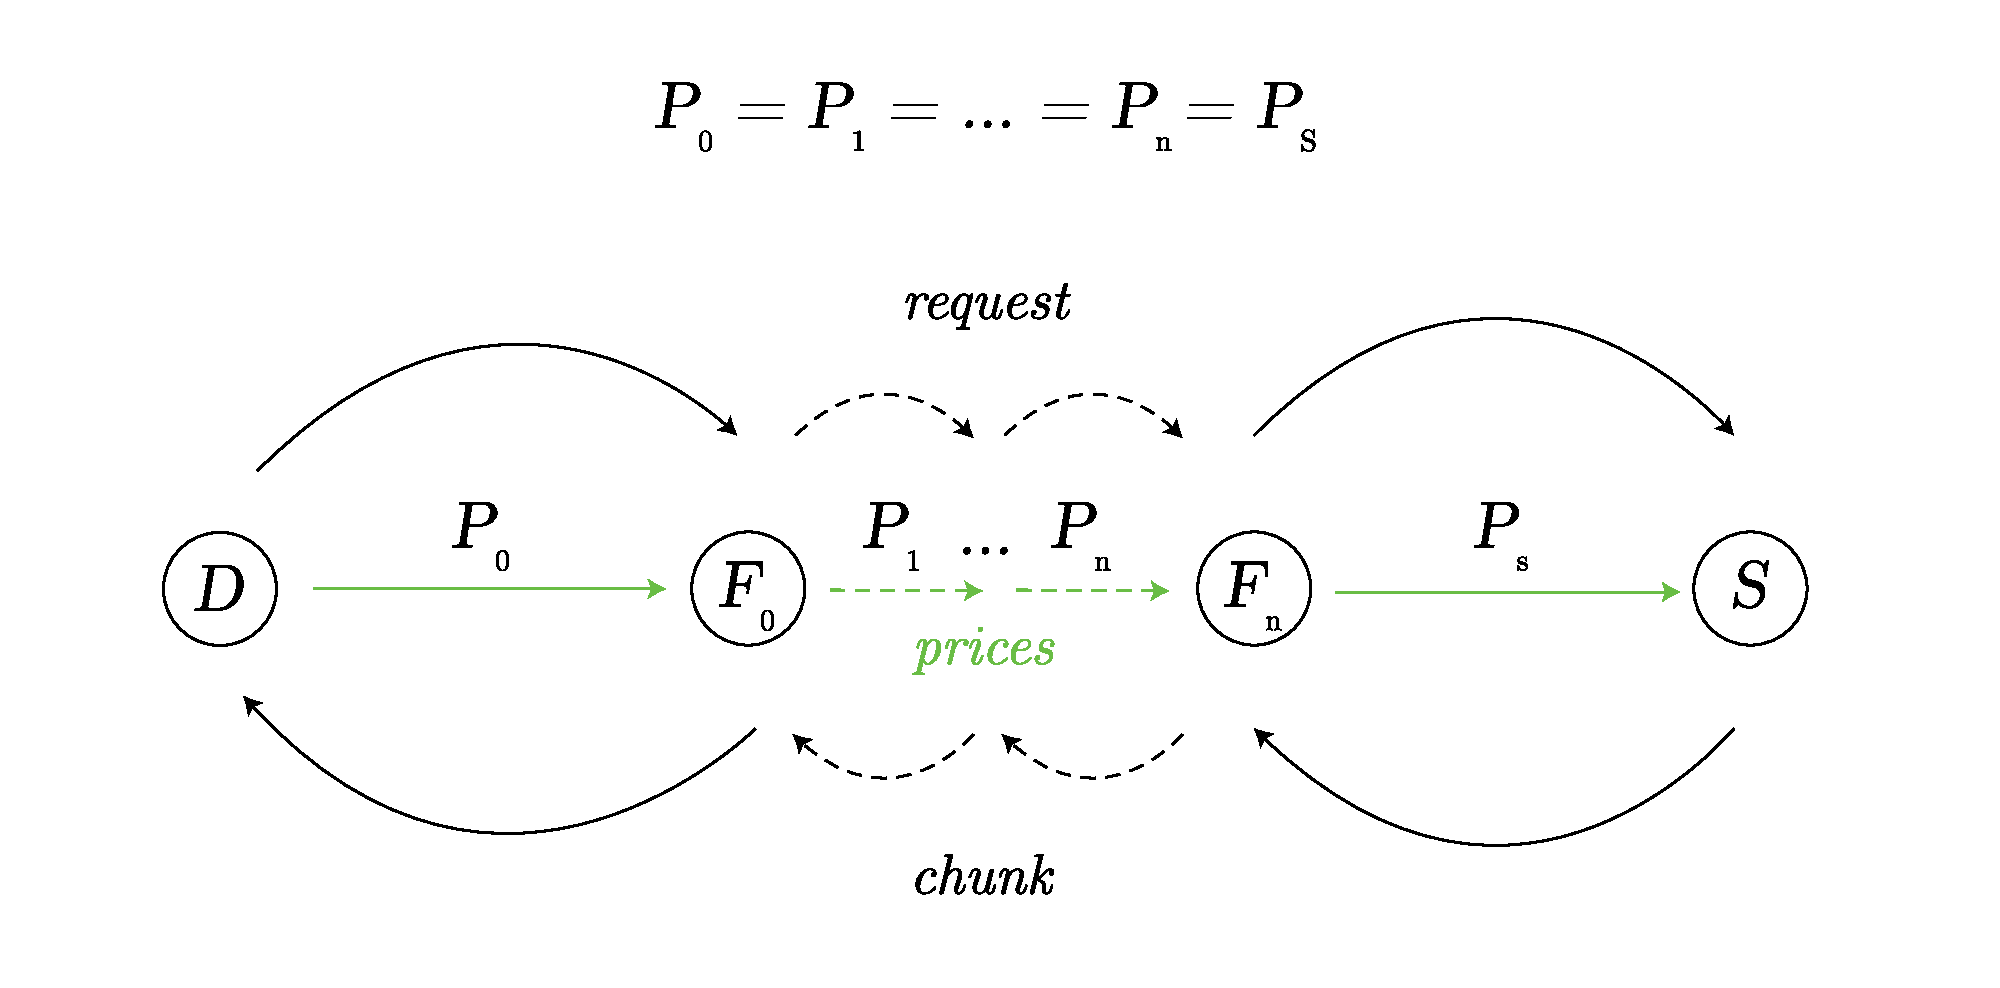
\includegraphics[width=\textwidth]{fig/ddos-uniform-price.pdf}
   \caption[Uniform chunk price across proximities would allow a DoS \statusgreen]{Uniform chunk price across proximities would allow a DoS attack. An attacker can create a flow of traffic between two nodes $D$ and $S$ by sending retrieve requests towards $S$ which only $S$ can serve. If prices are the same across proximities, such an attack would incur no cost for the attacker.}
   \label{fig:ddos-uniform-price}
\end{figure}

To mitigate this attack, the price a requestor pays for a chunk needs to be strictly greater than what the storer node would receive as compensation when a request is routed from requestor to storer. We need to have a pricing scheme that rewards forwarding nodes, hence, this necessitates the need for differential pricing by node proximity. If the price of delivery is lower as a node gets further from the chunk, then the request can always be sent that way because the forwarder will pocket the difference and therefore make a profit. This means that an effective differential scheme will converge to a pricing model where delivery costs more if the peer is further from the chunk address, i.e. rewards for chunk deliveries are a decreasing function of proximity. 

Due to competitive pressure along the delivery path and in the neighborhood, we expect that the differential a node is applying to the downstream price to converge towards the marginal cost of an instance of forwarding.
The downstream price is determined by the bin density of the node. Assuming balanced bins with cardinality $2^n$, a node can guarantee to increase the proximity order by $n$ in one hop. At the same time it also means that they can spread the cost over $n$ proximity bins pushing the overall price down.


\subsubsection{Uniformity of price across peers}

Take a node $A$ that needs to forward a request for a chunk which falls into $A$'s PO bin $n$. Notice that all other peers of $A$ in bins $n+1, n+2, ...$, just like $A$ also have the chunk in their PO $n$. If any of these peers, say $B$, has a price  for proximity order $n$ cheaper than $A$, $A$ can lower its price for PO bin $n$, forward all increased traffic to $B$ and still pocket the difference, see figure  \ref{fig:price-arbitrage}. Note that this is not ideal for the network as it introduces a \gloss{spurious hop} in routing, i.e., in relaying without increasing the proximity. 


\begin{figure}[htbp]
   \centering
   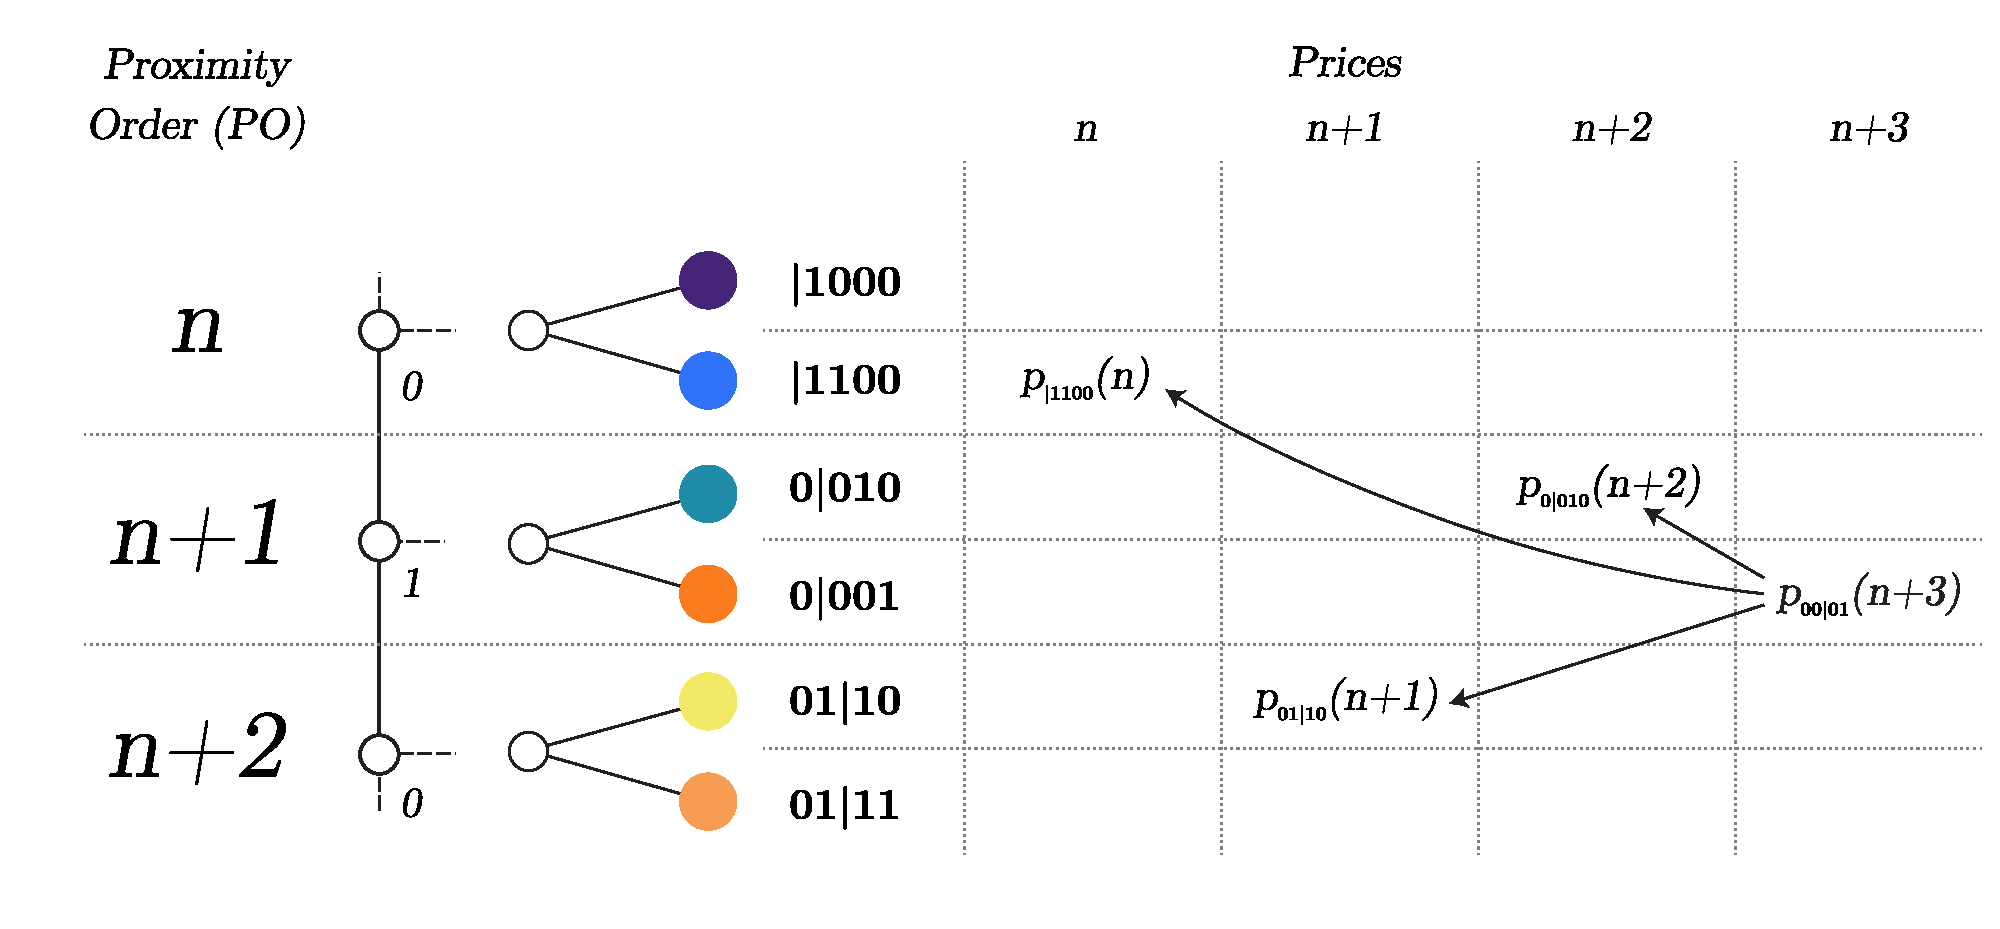
\includegraphics[width=\textwidth]{fig/price-arbitrage-3.pdf}


\section{Storage incentives \statusyellow}\label{sec:storage-incentives}

\wip{the lottery is not completely finalised}

In \ref{sec:postage-stamps}, we introduce \glossplural{postage stamp}, primarily as a measure for spam protection.  
Then, in \ref{sec:postage-lottery}, we turn to the \gloss{postage lottery}, explaining how postage stamps used for spam protection can be modified to create positive incentives for storer nodes to store files and for those uploading them to indicate their importance. In \ref{sec:capacity-pressure} we describe how the pricing mechanism can be used to signal capacity pressure of the network and how the incentives work to rectify this. Finally, \ref{sec:chunk-insurance} shows how the  positive rewards provided by the postage lottery can be complemented by introducing staked insurers who stand to lose their deposit if they lose  the chunks they have insured. We argue that such punitive measures are crucial in mitigating the \gloss{tragedy of commons} problem, which can afflict systems implementing positive storage incentives only. 

\subsection{Spam protection with postage stamps\statusgreen}\label{sec:postage-stamps}
\green{}

Syncing involves transferring chunks from the uploader to storers, i.e. from where they enter the network, to the neighbourhood where the chunk falls within the nodes' areas of responsibility. A storer node's role is to serve content by responding to retrieve requests with chunk data. All else being equal, given Kademlia routing, the closer a node is to the chunk address, the more likely it is that a request for that chunk will end up with them. This creates a weak incentive for storer nodes to sync content. However, it presupposes that the chunk has the promise of some profit. This assumption is not warranted if an adversary can spam the network with chunks (maybe randomly generated) that are never requested. From the network's point of view, this means that useless chunks would simply replace useful ones. By attaching a cost to uploading a chunk, Swarm can mitigate such an attack.


\subsubsection{Postage stamps}

Taking inspiration from international mail delivery, the entire delivery path (as well as storage) can be pre-paid. The proof of this payment is called a \gloss{postage stamp}, and must be attached to the payload by the sender.

This cost need not necessarily be borne by the uploader, but they are the ones that will need to make sure a postage stamp is attached to each chunk, otherwise the upload will not succeed. Conversely, this down-payment need not necessarily be paid out as revenue to anyone in particular, i.e. it could be burnt or otherwise redistributed. The actual cost of uploading a chunk can serve as a signal of its relative importance (somewhat analogously to priority mail), that storer nodes can then use to rank chunks when selecting which ones to retain and serve, and which ones to garbage collect (see \ref{spec:strategy:garbage-collection}) in the event of capacity shortage.

A postage stamp is modelled as a proof of payment associated with a chunk using a \gloss{witness}. The witness is implemented as a digital signature issued by a third party entity who is designated by the payer.


\begin{figure}[htbp]
\centering
  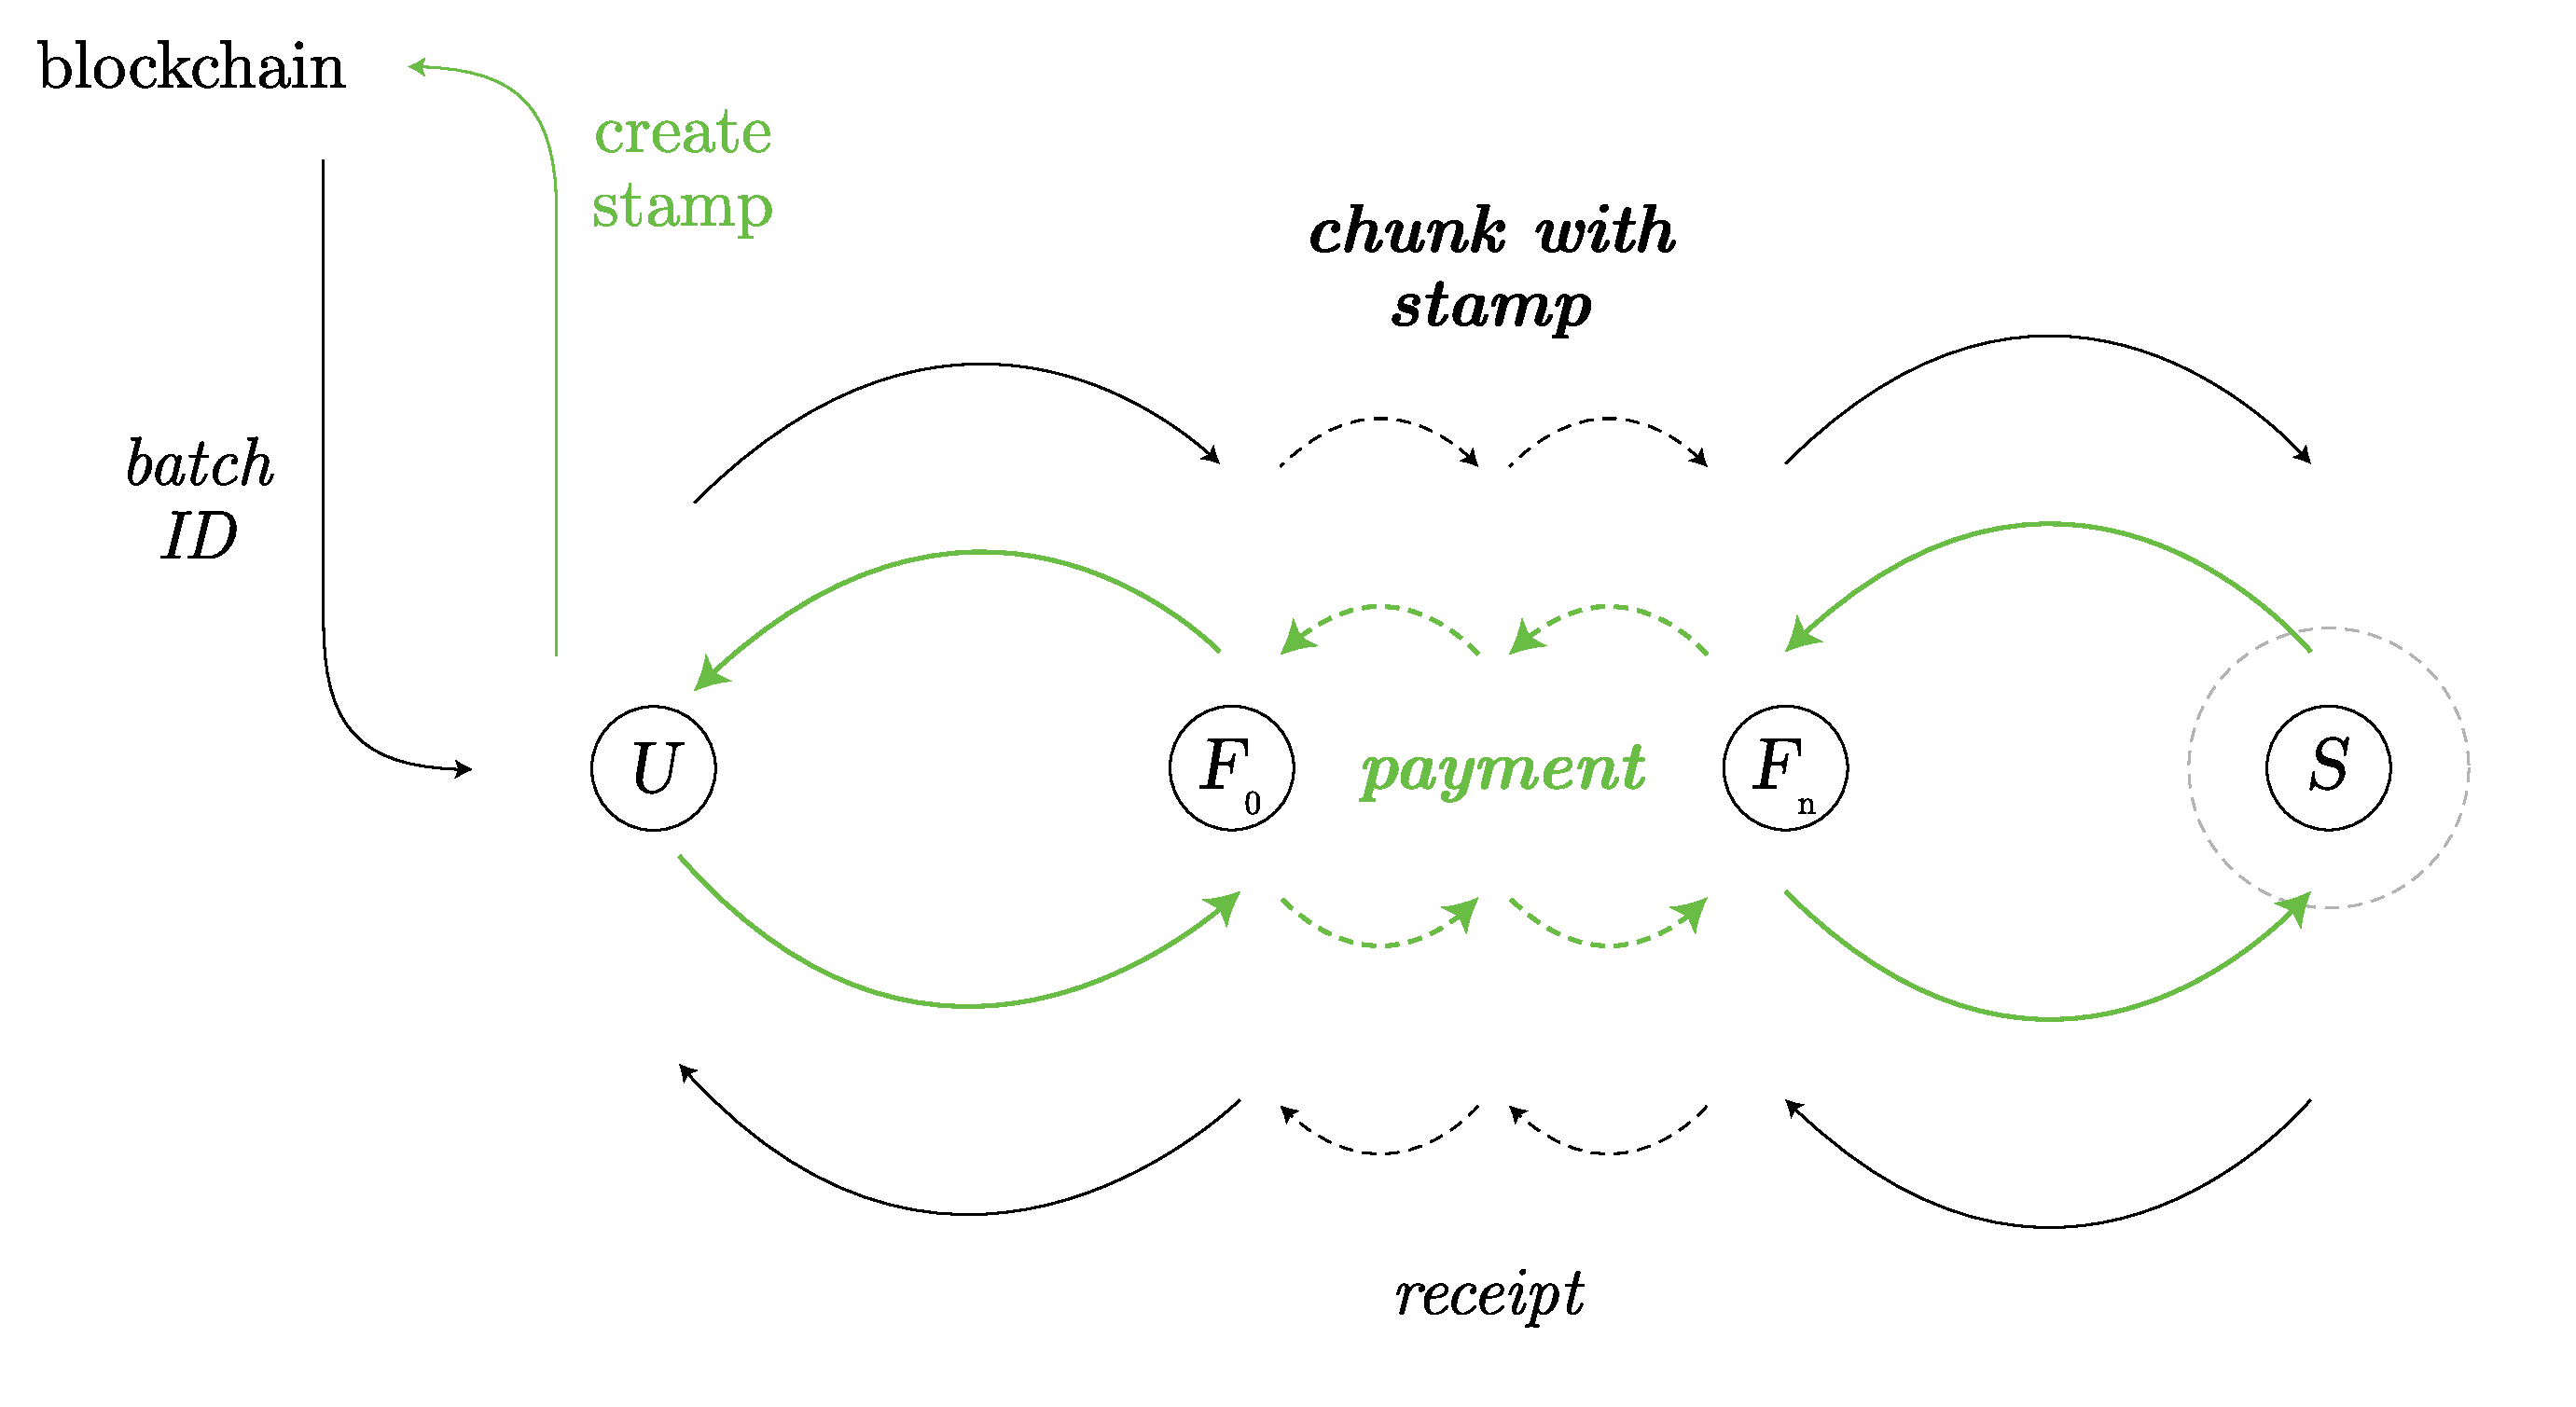
\includegraphics[width=\textwidth]{fig/postage-stamp.pdf}
\caption[Postage stamps  \statusgreen]{Postage stamps}
\label{fig:postage-stamps}
\end{figure}

\subsubsection{Proof of payment}

The proof of payment can lend itself to a number of different implementations. The most obvious choice is to make payments to a central postage stamp issuer smart contract on the blockchain.%
%
\footnote{Using a cheque seems like one option, however, since cheques are signed against cumulative debt and assume the single beneficiary is able to reconstruct the added value over the previously sent cheque. In other words, cheques are not an appropriate means to communicate value to non-peers.}
%
However, because of the high transaction cost, requiring an on-chain payment for each chunk would be prohibitively expensive. Instead, we need a solution that allows the uploader to purchase the postage stamps in a \gloss{postage batch} and then re-use it over many chunks. 


The batches are created by a central postage smart contract when a transaction is sent to its creation endpoint, together with an amount of BZZ tokens and the following transaction data:

\begin{itemize}
\item \emph{owner address} -- The owner that is entitled to use the batches created to stamp chunks.
\item \emph{batch depth} -- Logarithm of the number of chunks that can be stamped with each batch created.
\end{itemize}

This postage payment then results in the following information being recorded:

\begin{itemize}
\item \emph{payment reference ID} -- A random ID that is generated as reference for this payment.
\item \emph{per-chunk balance} -- The total amount, equally allocated for each chunk covered by this payment.
\item \emph{owner address} -- The owner that is entitled to use the batches created to stamp chunks.
\item \emph{batch depth} -- Logarithm of the number of chunks that can be stamped with each batch created.
\end{itemize}


The owner is the address that is specified in the transaction data and recorded as the party authorised to use the batches created to stamp chunks; if not specified, it is assumed to be the transaction sender by default. 

A random identifier is generated to provide a reference to the payment. The batch depth is recorded for each batch separately. The amount of BZZ tokens sent with the transaction is then allocated equally to all chunks covered by the payment, i.e. the total amount of tokens, divided by the number of chunks covered is assigned to the payment ID to represent the per-chunk balance of the batches. Anyone can then choose to top up this balance at a later date. 


\begin{figure}[htbp]
  \centering
    
\includegraphics[width=\textwidth]{fig/postage-stamp-structure.pdf}
  \caption[Postage stamp \statusgreen]{Postage stamp is a data structure comprised of the postage contract batch id, the chunk address and a witness signature attesting to the association of the two. Uploaders and forwarders must attach a valid postage stamp to every chunk uploaded. }
  \label{fig:postage-stamp}
\end{figure}


The postage stamp attached to a chunk is a data structure comprising the following fields (see figure  \ref{fig:postage-stamp}  and the specification in \ref{spec:format:postage-stamps}):

\begin{itemize}
    \item \emph{chunk address} -- The address the stamp is attached to. 
    \item \emph{batch identifier} -- Composed of a payment identifier and a batch index validity of which can be checked with the postage smart contract.
    \item \emph{witness} -- The owner's signature, linking the batch identifier and the owner's address.
\end{itemize}

The \emph{value} of a batch is the adjusted normalised balance associated with it.
Similarly to stamps used for postal mail, a single chunk can have multiple postage stamps attached to it. In this case the value conferred to the chunk by multiple valid postage stamps are added up to form the total postage stamp value. 

\subsubsection{Validity of postage stamp}

A postage stamp's validity can be checked by ensuring the following criteria are met:

\begin{itemize}
\item \emph{authentic} -- The batch identifier is valid, i.e. the payment ID exists and is registered, and the batch index is less than the number of batches associated with the payment ID.
\item \emph{authorised} -- The witness is signed by the address specified as the owner of the batch.
\item \emph{funded} -- The referenced batch has not yet exhausted its balance and is sufficiently funded to cover at least a single storage epoch for the latest  price.
\end{itemize}

All this can be easily checked by the smart contract itself. Validating that less than the total amount of chunks that are allowed to be stamped by a batch are contained within it is crucial. Without further measures, there could be a possibility for an overspend attack in which the uploader reuses the stamp over more chunks than the batch size would warrant and thereby trick the unsuspecting storers into underpaid extra work. 

Protection against such \emph{overissuance} is not trivial: In the absence of global visibility of all chunks signed with a particular batch, nodes cannot directly verify the size, as they have no access to postage stamps attached to chunks that are not relayed through them. Therefore, there needs to be a way for nodes to prevent overissuance collectively, while each must determine how to act based only on locally available information.

\subsubsection{Limiting batch size by constraining prefix collisions}

A solution is to impose an explicit \gloss{uniformity requirement} on the batches: a constraint that chunks signed with the same batch identifier have no \gloss{prefix collision} longer than the depth. A postage stamp with a batch size of $2^d$ can be thought of as a balanced binary tree of depth $d$, where the leaves correspond to maximum length \glossplural{collision slot} of the batch. If the depth of a batch is greater than the depth of the network (log of the number of nodes in the network), then all chunks matching the same collision slot are guaranteed to land in the same neighbourhoods, and, as a result, "violations" of the uniformity requirement can be locally detected by nodes (see figure \ref{fig:prefix-collision}). 
% If storers respond to this violation by randomly keeping only one of the chunks for each collision slot, uploaders will not only lose one chunk if they try to store more then their allowed allocation, but also lose the  predictability of which one on top.
Storer nodes then are expected to  correct the depth recorded with a batch.
They can do the correction by reporting two postage stamps issued by the owner against a batch that are closer than the currently recorded depth for the batch.
The incentive to do this comes from the possibility for a storer to obtain the extra storage cost above the one already paid out.


\begin{figure}[htbp]
  \centering
  \input{fig/prefix-collision}  \caption[Limiting the size of a postage stamp \statusgreen]{The postage batch is represented as a binary tree and is maps the stamps issued to the batch.  The leaf nodes are at a level from the root which corresponds to the depth of the postage batch as set at the time of payment. The boxes on the leaf nodes can be thought of as the prefix collision slots. In this figure, the gray boxes represent already filled slots, so the next chunk address should be made to fall into a white one.}
  \label{fig:prefix-collision}
\end{figure}


As chunk addresses are unlikely to be perfectly distributed over the collision slot of a batch, an uploader must keep more than one batch of depth $d$ to sign $2^d$ chunks. In general, the most efficient utilisation of each stamp is by filling all the different \glossplural{collision slot} (see \ref{sec:upload}). Put differently, continued non-uniformity will lead to underutilised stamps, and therefore a higher average unit price for uploading and storing each chunk. This solution has the desired side effect that it imposes an upfront cost to non-uniform uploads: the more focused our upload is on a neighbourhood, the more slots of the postage stamps remain unused. In this way, we ensure that directing too many uploads towards a particular neighbourhood is expensive.%
%
\footnote{The cost of targeted attacks DoS-ing neighbourhoods is exponential with depth.}
%
This will be significant for the later discussion of decentralised file insurance (see \ref{sec:insurance}). 

Another advantage of limiting batch size based on prefix collisions is that with prefix collisions, the absolute value of a postage stamp can be estimated. This comes in handy later when designing the postage lottery (see: \ref{sec:postage-lottery}). 


In order for these collisions to be detectable, the batch size needs to be higher than the estimated neighbourhood depth over the whole lifetime of the batch. In any case, it is not in the interest of users to have batches much deeper than that, since the longer the collision prefixes, the more difficult it becomes to achieve uniformity and fill the entire batch  (see \ref{sec:complexity-filling} of the appendix). 
% We will, for now, just assume that the depth of a batch is a fixed number set centrally in the contract and that follows the depth of Swarm. The effect of network growth on the already used stamps is discussed below.


\subsubsection{Mining chunks using encryption}

One neat solution to completely fill up \glossplural{postage batch} relies on the insight hinted at in \ref{sec:chunk-encryption}: Choosing the encryption key allows us to \emph{mine} a chunk to a specific postage batch.

The process of finding an encryption key to generate a content hash close to an address is analogous to mining blocks in a blockchain. Encryption of chunks requires a 32-byte key, which plays the role of the nonce in a block, that is: It provides enough entropy to guarantee that one is able to find an encryption key such that the hash digest of the resulting encrypted chunk produce an address which falls into a particular slot within an open postage batch. The difficulty of mining is determined by the batch depth. 

Consider the thrifty uploader that only has as many postage collision slots as chunks to send. Given a postage batch with depth $d$, they encrypt the chunk with a key chosen such that the resulting encrypted chunk's address fills a free collision slot of an open postage batch. As shown in the analysis found in appendix  (\ref{sec:complexity-filling}), this strategy of filling a batch requires an average of $0.69d+1$ trials per chunk, i.e. 8, 15, 22 for a thousand, million and billion nodes respectively. This is found to be of a reasonable complexity.


\subsection{Postage lottery: positive incentives for storage \statusyellow}\label{sec:postage-lottery}

\yellow{}

As discussed in \ref{sec:accounting}, an important incentive mechanism in Swarm is providing compensation for retrieval, where nodes are rewarded for successfully having served a chunk. This reward mechanism has the added benefit of encouraging opportunistic caching. Profit-maximising storage nodes serve chunks that are often requested from them and as a result, ensure that popular content becomes widely distributed across the network and thus also the retrieval latency is decreased.

The flipside of using only this incentive, is that chunks that are rarely retrieved may end up being lost: If a chunk is not being accessed for a long time, then as a result of limited storage capacity, it will eventually end up garbage collected to make room for new arrivals. In order for the swarm to guarantee long-term availability of data, the incentive system needs to make sure that additional revenue is generated for chunks that would otherwise be deleted. In other words, unpopular chunks that do not generate sufficient profit from retrievals should compensate the nodes that store them for their opportunities forgone. The \gloss{postage lottery} presented in this section provides such a compensation through redistributing the revenue coming from postage stamps among the storer nodes in a fair way.



Central to the postage lottery scheme is the realisation that probabilistic payments can be used to create revenue for storer nodes.
Using a lottery allows us to calibrate earnings that in the long run will have the same payout as if there was an actual payment for each chunk, yet save on transaction costs and provides the randomness which is necessary to serve as spot-checks.


\subsubsection{Race: raffle, apply, claim and earn}

The postage lottery takes place on an \gloss{EVM} blockchain and is managed by a smart contract. The lottery process is defined by the following protocol (see formally in \ref{spec:format:postage-stamps}). 

Every $N$-th%
%
\footnote{$N$ is chosen so that the period  between two rounds comfortably accommodates all phases of the lottery process.}
%
block on the blockchain marks the beginning of a new global lottery round.
The subsequent $N$ blocks are composed of three phases representing periods during which the participants in the raffle are expected to send transactions to interact with the raffle smart contracts: 

\begin{enumerate}
\item \emph{pre-committal} -- nodes pre-commit to the raffle challenge by sending in a price offer. As a result of valid pre-committal transactions, a set of applicants is defined. The end of this period is marked by the selection of the witness batches.
\item \emph{submission} -- nodes send a list of chunks and their proofs of custody as dictated by the witness batches. As a result of valid claim transactions, a set of claimants are defined. The end of this period is marked by the selection of challenges.
\item \emph{refutation} -- nodes send refutations of the challenges. As a result of valid refutations, a set of final prize winning claimants are determined. The end of this period is marked by the payout to the winners.
\end{enumerate}

The moment the last period ends a new raffle round begins. The lottery and its phases can also be characterised by the acronym \gloss{race}, with, of course, an mnemonic resolution detailing the phases: \gloss{raffle--apply--claim--earn}. The timeline of events is depicted in figure \ref{fig:raffle-timeline}.


\subsubsection{Automatic raffle rounds}

The RACE process is initialised with the raffle phase. First, the hash of the starting block is hashed together with integers from $0$ up to $n-1$ to obtain $n$ \emph{winning tickets} ($r_0, \ldots r_{n-1}$) each of which represents an independent \gloss{raffle draw}.%
%
\footnote{Multiple raffles each round are needed to calibrate the expected frequency for a node to win a raffle. By increasing $n$ as the network grows the expected time needed to get compensated for storage services can be kept constant.}. 
%
Once these winning tickets have been produced, nodes whose addresses are in the close proximity of the ticket $r_i$ are then able to apply to participate in the applicable raffle.


From the network perspective, these raffles serve as spot checks on storer nodes, whereas from the storer nodes' perspective, raffles represent the means of securing compensation for providing network storage within the swarm. 


\begin{figure}[htbp]
  \centering
  \includegraphics[width=\textwidth]{fig/postage_race.pdf}
  \caption[Timeline of events in a raffle round \statusgreen]{Timeline of events in a raffle round.}
  \label{fig:raffle-timeline}
\end{figure}


\subsubsection{Apply: precommit to raffle challenge}

In the first interactive phase, in order to apply for the prize, all nodes in the proximity of the winning ticket must send a transaction to the lottery contract including a price offer for storing a chunk per block. By submitting such a price, a node implicitly declares that it has in its possession all chunks of all batches with value higher than the price within their radius of responsibility. This radius of responsibility is self-claimed by the nodes and is part of the pre-committal. 

% \begin{figure}[htbp]
%   \centering
%   \includegraphics[width=.7\textwidth]{fig/radius_of_responsibility.pdf}
%   \caption[Radius of responsibility for postage lottery claims \statusorange]{Radius of responsibility for postage lottery claims}
%   \label{fig:raffle-radius}
% \end{figure}

\subsubsection{Claim: submit proofs to win}

After this application deadline has passed, the raffle enters into the claim phase by designating a \gloss{witness batch} for each applicant. This witness batch serves as a spot check for the applicant's claim that they store all the chunks that they are responsible for. Analogous to the winning tickets, the witness batch is selected based on randomness provided by the \gloss{blockhash} of the block that closes the application round $h_1$.  The spot check is implemented  by the following procedure. First create an anchor by hashing together the blockhash $h_1$ and the applicant's address, and then choose the batch which has the id closest to the anchor and has a value above the price submitted in the application. This batch serves as the random witness batch against which applicants will submit evidence that they are still in custody of all their allocated chunks. 

As we have discussed previously, stamps attached to a chunk endow that chunk with a value, as defined by the per-chunk balance of the batch. Pursuing a \gloss{value-consistent garbage collection strategy} (see \ref{spec:strategy:garbage-collection}) implies that the minimum postage stamp value accepted on a chunk will coincide with the storer node's garbage collection cutoff value. Nodes that follow this strategy faithfully, know that they have never deleted a chunk whose postage value was above their minimum required postage value. In this way, they can be confident that they are able to include all relevant chunks above that value, no matter which batch is selected to be the witness.

The claim phase is separated from the application phase exactly in order to force applicants to pre-commit to any spot check, since: if the witness was known at the time of application, frivolous nodes could simply claim the prize even if they just serendipitously stored only the chunks of the witness batch.  In  order to discourage such     opportunistic   behaviour, participation in the raffle requires a deposit sent  with the precommittal. This amount is added to the reward pool if the node fails to survive the remaining phases of  the raffle round, otherwise given back to the applicant.

To claim the raffle prize, a node must show that they have every witness chunk, i.e. every chunk stamped with the witness batch that falls within their radius of responsibility. In order to prove possession of chunk data, nodes must submit a \gloss{batch proof of custody}, a canonically ordered list of \glossplural{BMT proof} (see \ref{spec:format:bmt}), one for each witness chunk (see figure 
\ref{fig:batch-proof-of-custody}). Applicants have $N_2$ blocks to submit their claim, after which the raffle enters the challenge phase. Applicants that applied but failed to submit a claim are treated as if they had submitted an invalid claim.   


\begin{figure}[htbp]
  \centering
   \includegraphics[width=\textwidth]{fig/batch-proof-of-custody.pdf}
  \caption[Batch proof of custody \statusgreen]{Batch proof of custody. A Proof of custody is BMT inclusion proof wrapped with the chunk address, the segment index and the postage stamp. Multiple POCs are packaged with a witness batch id.}
  \label{fig:batch-proof-of-custody}
\end{figure}

\subsubsection{Earn: challenging the applicants}

% If the set of chunks presented to the blockchain is incomplete (i.e. it doesn't contain all chunks for which a statement of custody receipt was issued), the applicants can be challenged on the blockchain. The challenge contains a statement of custody receipt that was signed previously by the applicant (see \ref{sec:push-syncing} and \ref{sec:push-sync-incentives}). This receipt can then be submitted by any third party and is validated right away by the smart contract. If the challenge is valid, the applicant loses their registration immediately and more punitive measures may be enacted by his peers. Challengers have till the end of the raffle round to challenge applicants.

\subsubsection{Choosing the winner}

After the challenge phase ended ($N$ blocks after the beginning of the raffle round), from amongst the applicants that have survived the challenge period, for each raffle, the ones that offered the lowest prices will win the round. The  price itself is the lowest price that any of the neighbourhood's winners applied with.

The lottery prize payout needs to take into account the number of winners, the number of chunks, the proportion of a nodes' storage with respect to the total volume stored in Swarm.
The period that the payout is for is equally distributed among winners. For ease of reasoning, it is possible to calibrate blocks = winners, so that we can say a node when it wins gets paid for all chunks for a block. The winner is entitled to collect the price for each chunk whose price is not lower than the minimum required by the winner. The sum of all winners' proceeds is subtracted from the remaining balance of each batch. The postage batches whose balance is dried out after the payout are removed from the contract.%
%
\footnote{In practice, such a balance adjustment is unnecessary, see \ref{spec:format:postage-stamps}).
}

While winning nodes could try to benefit from a higher price for a bigger win, they are competing with each other to try to win the raffle, so they are incentivised to secure their win by offering the actual cutoff value they used for garbage collection. As a result of competitive payouts, it is expected that the unit prices will converge on the marginal cost of storing one more chunk plus storer/forwarder/challenger margins.




\subsubsection{Batch depth and volume adjusted payouts}

So far, for ease of reasoning, we assumed that the depth of each batch was given.  The requirements of batch depth are that it is deeper than the neighbourhood depth so that prefix collisions are always caught by storer nodes, yet not too much deeper so that it would make batches too difficult to fill completely (see \ref{sec:complexity-filling}). If a batch of depth $b$ has been filled completely, then a storer node with radius of responsibility $d$ is expected to store  $2^{b-d}$ chunks belonging to this batch.
Half of these with proximity of order $d$ to the winner's address. 

In order to incentivise $r$ redundant replicas of chunks, each stored at one of  the  nodes in a neighbourhood, winners are expected to store the same chunks. 
Moreover, partial storage of a batch's chunks should be discouraged. 
Both are  taken care of if nodes are incentivised to present the most chunks they possibly can for a batch.
This incentive translates to partial  storage of local chunks of a match leads to lower winnings. This is achieved if each batch detected depth as well as actual size are both reported as part of the precommit. Falsely committing to more chunks than stored by the node for a batch runs the risk of an unrefutable challenge on the batch (if designated as a witness) resulting in losing the price one-time raffle ticket on top of not earning  the raffle prizepool. All this aligns uploaders   and storers on attempting to use completely filled batc hes (the collision slots constituting a balanced binary tree of depth $b$.)
Since the actual sizes constitute an estimation of actual chunk volume is swarm. 

The best arrangement of storer is if the 
In particular we propose that a volume-adjustment scheme is used  when applicants 

This is implicit in the require
Conversely, based on the actual number of chunks per batch presented to the contract by winners, $C$ we can make an estimate of the current neighbourhood depth in Swarm as $d'\defeq b - \mathit{log}_2(C)$. This gives the chance for the lottery smart contract to serve as a depth oracle. The oracle value can also be used as the minimum depth for any postage batch in the raffle calculations. Note that if self-claimed depth of a batch can be lower than the typical neighbourhood depth, then nodes are expected to have at  most one chunk of a batch in their storage and therefore unable to report overissued batches. Therefore active batches has the minimum size of $2^{d+1}$.


Practically old completely filled postage batches can either be retained or the content they cover can be re-insured. In the former case, a node would want to retain the batch in case the network wide neighbourhood depth grows and exceeds the original depth of the batch, in which case the owner is able to add chunks to it legitimately. 
In order to add new chunks to a batch without collisions, one must remember the chunks they have already associated with the batch.%
%
\footnote{In fact is actually sufficient to just remember which collision slots were filled up to a depth that could possibly be reached by the growing network. In practice, as an optimisation, potential collision slots for depth  $b' >b$ can be recorded using a bit vector of length $2^{b'-1}$}
%

Note that owners can choose to pay an amount for postage that, even if the swarm grows a thousand fold, the balance would run dry only after a desired period. This becomes important in the context of \gloss{upload and disappear}.
Such deep batches require the same $O(\mathit{log}(n))$ computational overhead (see \ref{sec:complexity-filling}). This essentially means a discount   requiring  bulk purchase/use.





% \subsubsection{Statement of custody receipts}

% Statement of custody receipts are crucial in the lottery, as they enable nodes to challenge. The challenge constitutes of submitting a receipt signed by the applicant. It is either a chunk closest to the applicant or to one of its neighbours. If the challenge is valid, the applicant loses their registered status. 

% In order for syncing neighbours to be able to challenge, nodes need to attach a statement of custody receipt to all the chunks that they are closest to or that their neighbour peer is closest to. The peers can be sanctioned with disconnection and blacklisting in case of non-compliance. 

% As part of syncing, an aspiring storer node must sign statements of custody receipts for all the chunks that it is closest to. If the upstream peer did not require these, then they could not defend their territory as it were, i.e. they would have no grounds to challenge the new node when they apply for winning a raffle round after registering. Note that they do not need to keep all of the chunks, since one is enough to mount a challenge. Additionally, the upstream node is not incentivised to withhold chunks that belong to the new node as they cannot earn any lottery winnings from them once the new node enters the race. 

\subsubsection{Incentives implicit in the lottery}

This procedure incentivises nodes to adhere to the following behaviors:

\begin{itemize}
\item \emph{stay online} -- Otherwise the raffle is missed.
\item \emph{have a redundantly synced area of responsibility} -- Remain fully synced with their neighbourhood. Otherwise the claim may be incomplete and the volume-adjustment leaves the node with less.
\item \emph{have a fully indexed local store} -- To be able to list all chunks of a batch, nodes need to preserve postage stamps and keep an associated set of chunk addresses. 
\item \emph{perform value consistent garbage collection} -- In order to tell if the node locally stores all previously receipted chunks of a batch they must perform garbage collection value-consistently,%
%
\footnote{or store indexes of deleted chunks which is inefficient}
i.e. the minimum value accepted coincides with the maximum value ever deleted.
%
\item \emph{store the data} -- In order to provide BMT proofs the node must possess the data in the chunk content.%
%
\footnote{In the special case of addressed envelopes with pre-paid postage, no payout can be collected before the envelope has been filled and sent (see \ref{sec:addressed-envelopes}).}
\end{itemize}


\subsection{Price signalling capacity pressure \statusyellow}\label{sec:capacity-pressure}

\yellow{}

\subsubsection{Storage capacity}
Kademlia topology and the redundancy parameter determine the node's neighbourhood depth (see \ref{sec:redundancy-by-local-replication}). The neighbourhood depth delineates the area of responsibility. As a result of postage lottery, the nodes are incentivised to have a uniform neighbourhood size. The number of chunks uploaded to that area is simply proportional to the number of all chunks uploaded to Swarm $C$ and inversely proportional to the number of nodes in Swarm $N$. The number of chunks stored by a node is on average $CR/N$, where $R$ is the neighbourhood replication factor, measuring the degree of redundancy. This expresses the density of chunks in any neighbourhood. Given a particular connectivity and fixed storage quantity for a neighbourhood, $C/N$ captures the \emph{storage capacity pressure}. 

If we assume that chunks are meant to be preserved only for a limited period of time, then within some variance the pressure stays constant. In other words, we can find a network size%
%
\footnote{in the sense of storage capacity; or in the sense of number of nodes assuming a minimum storage capacity per node.}
%
such that all content that users want preserved is preserved. 

If the rate of new uploads to Swarm is higher than the rate of expiry (postage stamp balances going below the current price), then a fixed network will experience increasing pressure. As a consequence, without added capacity, after a while, content that is meant to be preserved will be garbage collected. 

Such capacity shortage is solved if added storage is invited by incentivising new storer nodes to join the network or rising demand is resisted by raising prices. Conversely, if the rate of expiry is faster than new uploads, pressure decreases and there may well be surplus capacity. The resulting situation with underutilised resources is remedied if added content is invited by incentivising users to upload their content or by some nodes dropping out disincentivised by lower prices. Thinking in terms of supply and demand, we can reach a self-regulating market simply if storage capacity pressure is signalled in the price of storage, i.e. the minimum value for postage stamp per chunk. 

\subsubsection{Garbage collection strategy and postage value}

The emergence of this self-regulating market is exactly what happens if we ensure that the garbage collection queue is prioritised by descending postage value (see \ref{spec:strategy:garbage-collection}).

\begin{figure}[htbp]
  \centering
  \includegraphics[width=\textwidth]{fig/garbage-collection-fixed.pdf}
  \caption[Garbage collection \statusgreen]{Garbage collection: chunks are ordered by profitability which comes from the postage value and a predicted retrieval revenue.}
  \label{fig:garbage-collection}
\end{figure}


Note that when a raffle round pays out, the same amounts get subtracted from all stamp balances. Therefore, the ordering by value does not change no matter how many raffle rounds have happened. However, in order to insert a newly created postage stamp, we will need to know the overall amount paid out so far and then add it to the new item's value.

A postage stamp must promise sufficient earnings with its value for the storer so that it outperforms the lowest quantile of competitors. When a node appends chunks to the bottom of the garbage collection queue, the postage value is updated by checking if there was a top-up on the blockchain.%
%
\footnote{In order to avoid checking updates on the blockchain for payout rate change, a node may just want to update the rate as a response to a payment event logged on the lottery contract.}
%
If there was a change, the chunk will need to be reinserted in the queue. 

\subsubsection{Combining retrieval popularity and postage value}

Besides expected lottery payouts, estimation of profitability needs to factor in earnings from serving popular chunks. If we record the number of times a chunk is served for every raffle \gloss{epoch}, then one can apply a predictive model to these datapoints to forecast the earnings for a future period. Fortunately, we only really need to decide which are the least profitable chunks. 

% The distribution of popularity is a power law distribution with a long  tail. Unless Swarm's capacity is so constrained that only popular chunks can be stored, we expect that nearly  half of chunks will not be accessed at all.


When we iterate over the chunks with the smallest postage value, we must decide if each chunk should survive the next epoch or if it has no real promise of being requested. The garbage collection process will then terminates once number of chunks matching the volume of a quantile have been deleted (see figure \ref{fig:garbage-collection}).

\subsubsection{Uniformity of prices} 

When push-syncing chunks, each forwarding node accepts chunks only if their postage value is higher than that node's advertised minimum. Practically this means that the initial postage value cannot be lower than the maximum such value in the network, otherwise syncing is not successful. This means that nodes keeping their postage price offer for the lottery low will not receive more traffic, they just have more chance of winning and need to have more storage capacity than their more expensive neighbours to be able to store the extra chunks whose value reached below their neighbour's minimum.

If neighbourhoods manage to keep their prices high, it will attract new nodes who will under-offer. If the high prices were genuine due to actual capacity shortage, then the new node adds storage space and corrects the non-uniformity. If the neighbourhood kept high prices because they cartellised, then the new node is able to disrupt this. Over a longer time period, therefore, prices are expected to converge.



% Whenever we serve a chunk we update the value of the chunk by adding the retrieval price. For the sake of simplicity, let us assume that there is the garbage collection cycle and the raffle round is at the same time. Knowing the earnings of the last epoch, we recalibrate the chunk profitability predictive model. 


